\documentclass[12pt,english]{article}
\usepackage[utf8]{inputenc}
\usepackage{graphicx}
\graphicspath{ {./images/} }
\usepackage{pdfpages}
\usepackage{amsmath}
\usepackage{amsfonts}
\usepackage{amssymb}
\usepackage{derivative}
\usepackage{cite}
\usepackage{enumitem}
\usepackage{caption}
\usepackage{dblfloatfix} %for moving figures
\usepackage{neuralnetwork}

\usepackage{fancyhdr}

\pagestyle{headings}

\setlength\parindent{0pt}

\usepackage[a4paper,bindingoffset=0.2in,left=1.25in,right=.75in,top=1in, bottom = 1in, footskip=.25in]{geometry}
\usepackage[margin=0.25in]{geometry} %graph plotting

\usepackage{tikz} %package for drawing NN
\usepackage{listofitems} %for drawing NN too 
\tikzstyle{mynode}=[thick,draw=black,circle,minimum size=22]
\renewcommand{\baselinestretch}{1.25} 
\newtheorem{example}{Example}

%below is for NN diagrams: 
% Author: Izaak Neutelings (September 2021)
% Inspiration:
%   https://www.asimovinstitute.org/neural-network-zoo/
%   https://www.youtube.com/watch?v=aircAruvnKk&list=PLZHQObOWTQDNU6R1_67000Dx_ZCJB-3pi&index=1
\documentclass[border=3pt,tikz]{standalone}
\usepackage{amsmath} % for aligned
%\usepackage{amssymb} % for \mathbb
\usepackage{tikz}
%\usepackage{etoolbox} % for \ifthen
\usepackage{listofitems} % for \readlist to create arrays
\usetikzlibrary{arrows.meta} % for arrow size
\usepackage[outline]{contour} % glow around text
\contourlength{1.4pt}

\tikzset{>=latex} % for LaTeX arrow head
\usepackage{xcolor}
\colorlet{myred}{red!80!black}
\colorlet{myblue}{blue!80!black}
\colorlet{mygreen}{green!60!black}
\colorlet{myorange}{orange!70!red!60!black}
\colorlet{mydarkred}{red!30!black}
\colorlet{mydarkblue}{blue!40!black}
\colorlet{mydarkgreen}{green!30!black}
\tikzstyle{node}=[thick,circle,draw=myblue,minimum size=22,inner sep=0.5,outer sep=0.6]
\tikzstyle{node in}=[node,green!20!black,draw=mygreen!30!black,fill=mygreen!25]
\tikzstyle{node hidden}=[node,blue!20!black,draw=myblue!30!black,fill=myblue!20]
\tikzstyle{node convol}=[node,orange!20!black,draw=myorange!30!black,fill=myorange!20]
\tikzstyle{node out}=[node,red!20!black,draw=myred!30!black,fill=myred!20]
\tikzstyle{connect}=[thick,mydarkblue] %,line cap=round
\tikzstyle{connect arrow}=[-{Latex[length=4,width=3.5]},thick,mydarkblue,shorten <=0.5,shorten >=1]
\tikzset{ % node styles, numbered for easy mapping with \nstyle
  node 1/.style={node in},
  node 2/.style={node hidden},
  node 3/.style={node out},
}
\def\nstyle{int(\lay<\Nnodlen?min(2,\lay):3)} % map layer number onto 1, 2, or 3

%END of NN diagrams 

%below is for code in appendices 
%START 
\usepackage{listings}
\usepackage{color}

\definecolor{dkgreen}{rgb}{0,0.6,0}
\definecolor{gray}{rgb}{0.5,0.5,0.5}
\definecolor{mauve}{rgb}{0.58,0,0.82}

\lstset{frame=tb,
  language=Java,
  aboveskip=3mm,
  belowskip=3mm,
  showstringspaces=false,
  columns=flexible,
  basicstyle={\small\ttfamily},
  numbers=none,
  numberstyle=\tiny\color{gray},
  keywordstyle=\color{blue},
  commentstyle=\color{dkgreen},
  stringstyle=\color{mauve},
  breaklines=true,
  breakatwhitespace=true,
  tabsize=3
}
%END 


\begin{document}

%START Title Page
{\centering{
\includegraphics[scale = 0.5]{LincolnLogo(1)}} \par}
\begin{center}
\newline\newline
\thispagestyle{empty}
\\[40pt]
    \textbf{\huge{Mathematics of Image Processing and Recognition}} \\[40pt] \Large{Adelaide Baron\\BAR16630927} 
     \\[20pt]{05/2022}
    \textbf{\\[130pt]\LARGE{Supervised by Dr Matthew Watkins}}
    \\[40pt]{Scientific Report in the Mathematics Module Project
    \\ MTH3001M}
\end{center}
%END Title Page 

%START Abstract
\newpage
\begin{center}
\textbf{Abstract}
\end{center}
This project aims to provide the reader with an understanding of the mathematics behind image processing and recognition, focusing on the particular case of handwritten digits zero to nine. We begin with an in-depth study of neural networks, their history, architecture, and the learning process of categorising images. We briefly visit the topic of coding such networks and the variety of available networks, and how they may impact the process. Afterwards, we visit edge detection filters and how these may be used in image processing to enhance images. Finally, we discuss interpolation methods such as Chebyshev Polynomials. 



%START TABLE OF CONTENTS
\newpage
\tableofcontents 
%END TABLE OF CONTENTS 

\newpage
\section{Introduction}
Photographs have been used for almost two hundred years to record memories. Initially taking around 20 minutes for a picture, considering time for exposure, photography was a luxury reserved for life events. Today, in the age of computers, cameras are easily accessible and developed, and so we use images to record information. From number plate recognition to CCTV, data is extracted from the images captured, where it is then stored and manipulated for development. The human eye can identify and classify information from the images - but how do we train computers to do so? This project aims to understand how we may use mathematics to process and classify images. We will strip back the recognition and classification process to the core of handwritten digit recognition. Once a method is developed to classify digits correctly, we may extend it to characters and symbols. It is then not a far stretch to develop these processes to recognise digits, characters, and symbols within images, with uses such as number plate recognition. \\ 


Throughout my undergraduate studies, I have used an electronic tablet and stylus to write my notes as I can search a word in my files to bring back all matches. When writing my early notes for this project, I wondered how the tablet recognised what I had written? Upon research, I found that neural networks are a popular method to classify digits, with success rates of over 97\% \cite{NN}. We begin this project with the history of neural networks (NN) and the earliest forms to understand the process. Once this is established, we move on to the architecture of artificial neural networks (ANNs), developing an understanding of each component and its impact on the classification process. The project then shows the reader an example of digit recognition using ANNs. \\

Once the reader understands an ANN and its structure, we explore activation functions. The ANN functions are used to adjust the data passed through to the output. In the next section, we explore the learning process of ANNs and how they take previously classified data to adjust their network to correctly classify unseen images. We culminate our focus on ANNs with a section on coding the ANNs, using languages such as C++ and Python to automate the process using the mathematical basis developed. Before moving away from neural networks, we explore the different types of NN. We focus primarily on ANNs, but we acknowledge Recurrent neural networks and convolutional neural networks to understand the differences and how we may take this project further with future studies. This section also discusses ways to generate digits with the NNs, primarily autoencoders and generative adversarial networks. The topic of neural networks deviates from mathematics to the topic of computer science. So we compare NNs with processes such as Edge Detection Filters (EDF) and interpolation. \\

Starting with EDFs, within this section, we acknowledge the Sobel Filter, which gave the initial motivation for me to take on this project \cite{SobelFilter}, as discussed in my research plan. In the next section, we explore interpolation, starting with Lagrange interpolation. Once the reader has a strong foundation of interpolation, we move on to the method of Chebyshev polynomials and a brief overview of their use in image classification. \\

We finish the report with a section on creating datasets before our conclusion discussing future opportunities from this project and assessing the contents explored. 

%\subsection{Key/references (look @ past reports for this)}
%\begin{itemize}
%\item \textbf{Interface}: tool used to draw on. For example, writing characters on paper, the paper is the interface. %This may be digital too. 
%\end{itemize}

\newpage


\subsection{Literature Review}

The main book I used to develop my understanding of neural networks and handwriting recognition was "\textbf{Neural Networks and Deep Learning}" by Michael Nielsen \cite{NN}. This book explores the development of NNs, the mathematics of the learning process, and derivation of. This book is referenced greatly in the online community for creating programmes for handwriting recognition. As a result, however, this book does too focus heavily on the programming of such NNs.  \\ 

As the overall topic of neural networks centres around programming languages, it was difficult to find physical text to describe the processes, rather than links to online resources.  \\ 

Another main book that I used for my understanding of neural networks and their structure was "\textbf{Machine Learning: An Algorithmic Perspective}" by Stephen Marsland \cite{Marsland}. Focussing more on the structure NNs, and the mathematics and statistics supporting it. Marsland's work was supported in other texts, such as "How many hidden layers and nodes?" by D. Stathakis \cite{Stathakis}. Additionally, Marsland touches upon the topic of interpolation and basis functions, once again giving a good overview of the topic as a whole.  \\ 

The main paper inspiring our focus on Chebyshev polynomials and interpolation overall was "\textbf{Representing and Characterizing Handwritten Mathematical Symbols through Succient Functional Approximation}" by Burce Char and Stephen Watt \cite{Chebyshev}. This paper also explores the development of Chebyshev polynomials for character recognition, modelling handwriting as strokes and capturing the shape of handwriting. It also references the InkML programme, which allowed me to explore documentation produced by W3C to explain the syntax and process \cite{INKML}.  \\ 


\subsection{Data Sets}  \label{datasets}
Throughout this project we will use data from the MNIST database \cite{MNIST}. This is a set of handwritten digits by National Institute of Standards and Technology including digits from employees of United States Census Bureau, and students in highschool. We split datasets into training and test data. The training set is used to improve the network, and the test data is used to test if the ANN learned as expected from the training data. We will discuss later, in section \ref{gatheringdataset}, how we may go about collecting our own data set. 

\newpage
\section{ANN: An Introduction} \label{structure}
% Rumelhart, David E., et al. "The basic ideas in neural networks." Communications of the ACM, vol. 37, no. 3, Mar. 1994, pp. 87+. Gale Academic OneFile, link.gale.com/apps/doc/A15061351/AONE?u=anon~a4799958&sid=googleScholar&xid=aeadf30e. Accessed 28 Mar. 2022.

Our brains work using biological networks between neurons. Neurons fire, triggering others to fire, akin to a chain reaction. These chain reactions are how the brain works, from controlling our senses to moving our muscles. Artificial neural networks (ANN) are modelled loosely on this biological process.\\ 


Like the brain, ANNs consist of neurons and connections. We will explore the structure of an ANN in section \ref{structure}. For now, consider figure \ref{basicANN}; showing the neurons (colourful circles), and the connections (lines). \\  

In this report, when I refer to neural networks unless specified otherwise, I mean artificial neural networks. Additionally, some texts refer to neurons as nodes, but we will retain the term neuron. 

%%BEGINNING OF NN DIAGRAM 
\begin{figure}[h] %can't get this to move to bottom of page 
    \centering

%adapt the following to be a different NN 
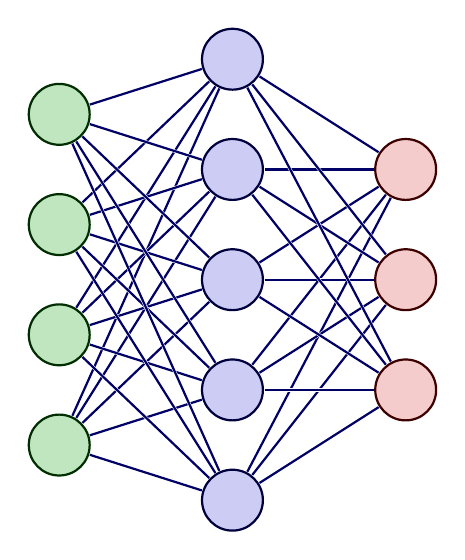
\begin{tikzpicture}[x=2.2cm,y=1.4cm]
  \message{^^JNeural network without text}
  \readlist\Nnod{4,5,3} % array of number of nodes per layer
  
  \message{^^J  Layer}
  \foreachitem \N \in \Nnod{ % loop over layers
    \def\lay{\Ncnt} % alias of index of current layer
    \pgfmathsetmacro\prev{int(\Ncnt-1)} % number of previous layer
    \message{\lay,}
    \foreach \i [evaluate={\y=\N/2-\i; \x=\lay; \n=\nstyle;}] in {1,...,\N}{ % loop over nodes
      
      % NODES
      \node[node \n] (N\lay-\i) at (\x,\y) {};
      
      % CONNECTIONS
      \ifnum\lay>1 % connect to previous layer
        \foreach \j in {1,...,\Nnod[\prev]}{ % loop over nodes in previous layer
          \draw[connect,white,line width=1.2] (N\prev-\j) -- (N\lay-\i);
          \draw[connect] (N\prev-\j) -- (N\lay-\i);
          %\draw[connect] (N\prev-\j.0) -- (N\lay-\i.180); % connect to left
        }
      \fi % else: nothing to connect first layer
      
    }
  }
\end{tikzpicture}

\caption{Artificial Neural Network}
    \label{basicANN}
\end{figure}
%%END OF NN DIAGRAM 



\subsection{History}
% https://en.wikipedia.org/wiki/Neural_network
%brief history of NNs, mention perceptrons - will return to these 

Biological neural networks were first observed and discussed in the late 1800s by Alexander Bain \cite{Bain} and William James \cite{James}. Until the 1940s, neural networks remained a purely biological concept. However, work by McCulloch and Pitts \cite{mcculloch} on neural network algorithms translated the theory into mathematics; leading to networks such as perceptrons (section \ref{Perceptron}) and the theory of ANN as we know it today. 

\subsubsection{Perceptrons} \label{Perceptron}

Perceptrons, depicted in figure \ref{perceptron_figure}, were the first mathematical neural networks to be proposed; named and studied by Rosebnblatt in 1962 \cite{NNforPC}. The perceptron is used often as a binary classifier. However, we will see in section \ref{BSF} that this is not the most practical for image recognition. To understand why, let's consider an example \cite{NNforPC} \cite{FirstNNbegin}. \\

\begin{figure}[h] 
\centering 
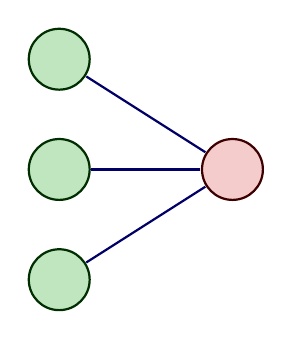
\begin{tikzpicture}[x=2.2cm,y=1.4cm]
  \message{^^JNeural network without text}
  \readlist\Nnod{3,1} % array of number of nodes per layer
  
  \message{^^J  Layer}
  \foreachitem \N \in \Nnod{ % loop over layers
    \def\lay{\Ncnt} % alias of index of current layer
    \pgfmathsetmacro\prev{int(\Ncnt-1)} % number of previous layer
    \message{\lay,}
    \foreach \i [evaluate={\y=\N/2-\i; \x=\lay; \n=\nstyle;}] in {1,...,\N}{ % loop over nodes
      
      % NODES
      \node[node \n] (N\lay-\i) at (\x,\y) {};
      
      % CONNECTIONS
      \ifnum\lay>1 % connect to previous layer
        \foreach \j in {1,...,\Nnod[\prev]}{ % loop over nodes in previous layer
          \draw[connect,white,line width=1.2] (N\prev-\j) -- (N\lay-\i);
          \draw[connect] (N\prev-\j) -- (N\lay-\i);
          %\draw[connect] (N\prev-\j.0) -- (N\lay-\i.180); % connect to left
        }
      \fi % else: nothing to connect first layer
      
    }
  }
\end{tikzpicture}
\caption{Perceptron}
\label{perceptron_figure}
\end{figure}

%book on Perceptrons https://en.wikipedia.org/wiki/Perceptrons_(book) 

%wiki perceptrons 
%https://en.wikipedia.org/wiki/Perceptron



\begin{example} \label{percep_example}
%correct term? boolean or binary
\noindent Consider a network with two boolean inputs and outputs, 0 and 1. The output depends on the inputs, with the following rule: 

\begin{center}
\begin{tabular}{||c c c||} 
 \hline
 Neuron A & Neuron B & Output \\ [0.3ex] 
 \hline\hline
 1 & 1 & 1  \\ 
 \hline
 1 & 0 & 1  \\
 \hline
 0 & 1 & 1  \\
 \hline
 0 & 0 & 0  \\ [1ex] 
 \hline
\end{tabular}
\end{center}

This may be modelled using a NN, similar to figure  \ref{perceptron_figure}. \\ 

Later in this report, section \ref{coding_nn}, we will explore coding such a network. You can see the results in the appendices,\ref{simpleNN}.
\end{example}

\newpage
\section{ANN: Structure } \label{structure}
Neural networks consist of two main components; layers, and weights. Within layers there are neurons, each with an associated bias. Information is passed forward from one layer to the next, and the weights affect this information transfer. As mentioned earlier, a generic NN looks like figure \ref{basicANN}. 

\subsection{Layers \label{layers}}
Layers are the columns of neurons in an ANN, and each one has a particular purpose. The first layer (left) is called the input layer, the last (right) is called the output layer, and those in between are hidden layers, as shown in figure \ref{ANNlayers}. The values of neurons in a layer, (L-1), determines the values of neurons in the next layer, L.  
%do more research, e.g. maths behind these numbers : 

\subsubsection{Number of Layers in a Network } \label{NoOfLayers}
When designing an ANN, we need to consider the optimal amount of hidden layers. The more layers, the longer the potential processing time may be. However, more layers may also allow for more sophisticated learning. This varies depending upon needs, and can come down to trial and error. However, a general rule for the amount of layers \cite{Java}: 
\begin{enumerate}
\item[i.] 0 Hidden layers - used for simple decisions, such as perceptrons. 
\item[ii.] 1 Hidden layer - used for simple mappings $X \mapsto Y $, both $X$ and $Y$ finite. Can be used within handwriting recognition, but restricts learning and may take longer to train. 
\item[iii.] 2 Hidden layers - used to represent functions of any shape. 
\end{enumerate}
You may see ANNs with more than two, but this is not practical within this project. 

\subsubsection{Referencing layers}
We adopt the following approach to referencing layers, indexing from the output layer backwards: 
\begin{itemize}
\item Output = L 
\item Hidden layers = L -  (number of layers between this layer and the output, L) - 1 
\item Input = L - (amount of hidden layers) - 1,  
\end{itemize}
When labelling components of an ANN, such as a weight or a neuron, we use a superscript to denote the layer, for example: $w^L, n^L$. 

\begin{figure}[htp] 
\begin{center}
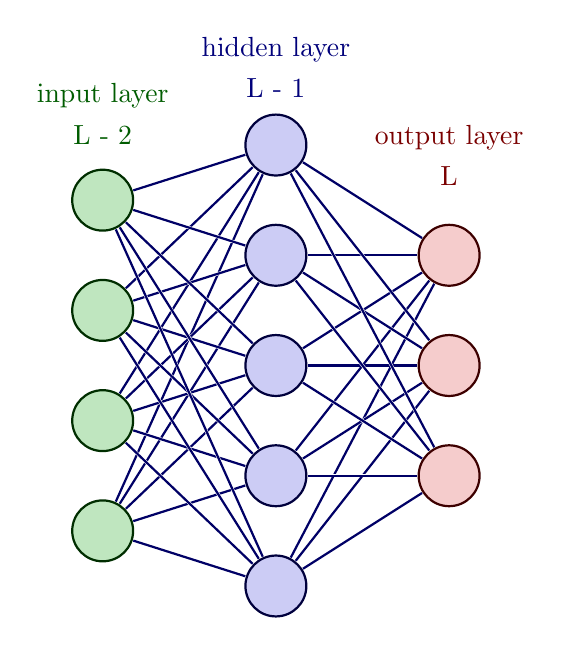
\begin{tikzpicture}[x=2.2cm,y=1.4cm]
  \message{^^JNeural network without text}
  \readlist\Nnod{4,5,3} % array of number of nodes per layer
  
  \message{^^J  Layer}
  \foreachitem \N \in \Nnod{ % loop over layers
    \def\lay{\Ncnt} % alias of index of current layer
    \pgfmathsetmacro\prev{int(\Ncnt-1)} % number of previous layer
    \message{\lay,}
    \foreach \i [evaluate={\y=\N/2-\i; \x=\lay; \n=\nstyle;}] in {1,...,\N}{ % loop over nodes
      
      % NODES
      \node[node \n] (N\lay-\i) at (\x,\y) {};
      
      % CONNECTIONS
      \ifnum\lay>1 % connect to previous layer
        \foreach \j in {1,...,\Nnod[\prev]}{ % loop over nodes in previous layer
          \draw[connect,white,line width=1.2] (N\prev-\j) -- (N\lay-\i);
          \draw[connect] (N\prev-\j) -- (N\lay-\i);
          %\draw[connect] (N\prev-\j.0) -- (N\lay-\i.180); % connect to left
        }
      \fi % else: nothing to connect first layer
      
    }
  }
  
  % LABELS
  \node[above=5,align=center,mygreen!60!black] at (N1-1.90) {input layer \\ L - 2};
  \node[above=2,align=center,myblue!60!black] at (N2-1.90) {hidden layer \\ L - 1};
  \node[above=10,align=center,myred!60!black] at (N\Nnodlen-1.90) {output layer \\ L };
  
\end{tikzpicture}
\caption{ANN layers}
\label{ANNlayers}
\end{center}
\end{figure}

\subsection{Neurons \label{neurons}}
Neurons sit within layers and have individual values. In the input layer, there is generally one neuron for each input value. In diagrams, such as figure \ref{ANNlayers}, the circles are the neurons. 

\subsubsection{Number of Neurons in a Network  \label{noOfNeurons}}
Like layers, the amount of neurons in a network is down to the creator, and depends on the requirements of the network. For the output, each neuron may represent a certain outcome, and thus we would have $n$ neurons for $n$ outputs.\\ 


For the case of handwriting recognition, we generally consider a 28 x 28 pixel image. So, with 784 inputs, we have 784 input neurons. We will consider 10 outputs, classifying the digits $[0,9]$. \\ 

The amount of neurons within hidden layers, we denote $n_{hidden}$ is more varied. Some people may make a decision based on aesthetics or at random \cite{NN}, but there are some popular rules to follow \cite{Stathakis} \cite{Java}: 
\begin{enumerate}
\item[i.] $n_{hidden}$ between $n_{input}$ and $n_{output}$
\item[ii.] $n_{hidden} = \frac{2}{3}$ ( $n_{input} + n_{output}$) 
\item[iii.] $n_{neuron} < 2|n_{input}$
\end{enumerate}

\subsubsection{Referencing neurons }
When referring to parts of an ANN, we use a subscript to denote the neuron index. We index from the top, n = 1, and work downwards. The indexing resets for each layer. 

\begin{example} \\ 
The 5th neuron in layer L-2 is $a^{L-2}_5$ \\ 
The 5th neuron in layer L-1 is $a^{L-1}_5$ 
\end{example}


% consider TESTING THE OPTIMAL NEURONS ETC 

\subsubsection{Activation} \label{activation}
%should this have it's own subsection? Or be within the neuron subsection (and be a subsubsection)? 

The numerical value of a neuron in an ANN is called the activation. In some cases, the value determines whether or not the neuron activates (for example, section \ref{activationFunction}). \\ 

We typically refer to an activation as $a$, and reference them the same way as neurons. We may also refer to the activations of the neurons in the output layer as $t^L$, and the desired output as $y^L$. \\ 

Within this project, the activation of neuron $n$ in layer $L$, $a_n^L$  depends upon the the product of activations and weights (\ref{weights}), added to the bias (\ref{biases}), in layer $L-1$. I.e.: $a^{L-1}_1 w_{n1} + a^{L-1}_2 w_{n2} + ... + a^{L-1}_m w_{nm} + b^L_n $, which we denote $z_n^L$. I.e.: 

\begin{equation} \label{zL}
z_n^L = a^{L-1}_1 w_{n1} + a^{L-1}_2 w_{n2} + ... + a^{L-1}_m w_{nm} + b^L_n  
\end{equation}

\noindent where $m$ = amount of neurons in layer (L-1), $w$ and $b$ are the weights and biases, discussed in sections \ref{weights} and \ref{biases}. \\ 

To aid the network in feeding forward values, it is typical to use an activation function, a function of $z^L_n$. We will explore this more in section \ref{sigmoid}, but in this report we restrict activation values to the range $[0,1]$ using the sigmoid function, defined as follows: 

\begin{equation} \label{sigmoidEqn}
 \sigma(x) = \frac{1}{1 + e^{-x}}
 \end{equation}
 where $x \in \mathbb{R}, \sigma \in [0, 1]$. I.e. $a_n^L = \sigma(z_n^L)$. \\ 

In a single layer, the neuron with the highest activation is referred to as the \textbf{brightest}. The brightest neuron in the output layer is the 'choice' of the network. \\

\subsection{Weights \label{weights}}

The connections between neurons in different layers are given weights. Increasing the weight between connections gives that specific connection more impact. 

\begin{example} 

Consider a section of an ANN where we have two neurons, $a^{L-1}_n$ and $a^{L-1}_m$,  connected to $a^L_j$, with respective weights $w^L_{jn}$ and $w^L_{jm}$. For simplicity, assume that these are the only three neurons, and we won't use an activation function. So,  $a^L_j =  w^L_{jn} a^{L-1}_n  + w^L_{jm} a^{L-1}_m$. Increasing the value of $w^L_{jn}$ will increase the impact of $a^L_{n-1}$ on the output, $a^L_j$. 
\end{example}

Thus, the higher a weight, the more influence that particular connection has on the end result. When we introduce the activation function, the relationship is no longer linear, but it remains positive. 

\subsubsection{Number of Weights in a Network }
A neuron in layer $L-1$ has $n+m$ associated weights, where $n = |L-2|$, $m = |L|$. 

\subsubsection{Referencing Weights}
We adopt a similar process as we do for neurons, but with two indices rather than one. A weight connecting the $k$th neuron in $L-1$ to to $j$th neuron in $L$ is $w^L _ {jk}$ 

\subsection{Bias} \label{biases}
A bias adds more impact to a particular neuron. It is added on to the value of the weights combined with activations, and each neuron has only one bias. Revisiting equation \ref{zL}: 
$z_n^L = a^{L-1}_1 w_{n1} + a^{L-1}_2 w_{n2} + ... + a^{L-1}_m w_{nm} + \textbf{b}^L_n $. 

\subsubsection{Number of Biases in a Network }
There is one bias per neuron. E.g. for a four-layer network with ten neurons in each, there are forty biases. 

\subsubsection{Referencing Biases}
Biases are referenced the same as neurons, but $b$ rather than $n$. I.e. $b^L_j$ \\

\newpage
\subsection{Example }

I am going to demonstrate the structure of an ANN with a handwriting recognition example, referring to figure \ref{NNHandwriting}. We will refer to this network throughout the report. 

\begin{example} \label{handwritingEG}
We consider pictures that are 28 x 28 pixels so that our ANN is compatible with the MNIST database \cite{MNIST}.  \newline

\begin{figure}[htp] 
\centering
% NEURAL NETWORK with coefficients, shifted
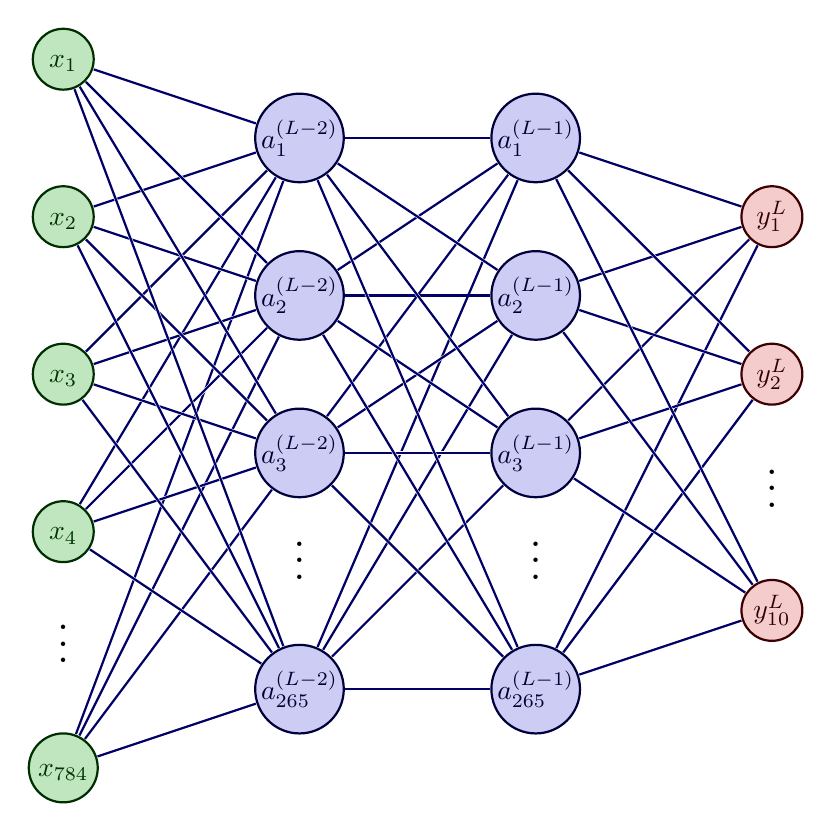
\begin{tikzpicture}[x=3cm,y=2cm]
  \message{^^JNeural network, shifted}
  \readlist\Nnod{5,4,4,3} % array of number of nodes per layer
  \readlist\Nstr{784,265,265,10} % array of string number of nodes per layer
  \readlist\Cstr{\strut x,a^{(L-2)},a^{(L-1)},y^{L}} %labels of neurons
  \def\yshift{0.5} % shift last node for dots
  
  \message{^^J  Layer}
  \foreachitem \N \in \Nnod{ % loop over layers
    \def\lay{\Ncnt} % alias of index of current layer
    \pgfmathsetmacro\prev{int(\Ncnt-1)} % number of previous layer
    \message{\lay,}
    \foreach \i [evaluate={\c=int(\i==\N); \y=\N/2-\i-\c*\yshift;
                 \index=(\i<\N?int(\i):"\Nstr[\lay]");
                 \x=\lay; \n=\nstyle;}] in {1,...,\N}{ % loop over nodes
      % NODES
      \node[node \n] (N\lay-\i) at (\x,\y) {$\Cstr[\lay]_{\index}$};
      
      % CONNECTIONS
      \ifnum\lay>1 % connect to previous layer
        \foreach \j in {1,...,\Nnod[\prev]}{ % loop over nodes in previous layer
          \draw[connect,white,line width=1.2] (N\prev-\j) -- (N\lay-\i);
          \draw[connect] (N\prev-\j) -- (N\lay-\i);
          %\draw[connect] (N\prev-\j.0) -- (N\lay-\i.180); % connect to left
        }
      \fi % else: nothing to connect first layer
      
    }
    \path (N\lay-\N) --++ (0,1+\yshift) node[midway,scale=1.5] {$\vdots$};
  }
  
  % LABELS
%  \node[above=5,align=center,mygreen!60!black] at (N1-1.90) {input\\[-0.2em]layer};
 % \node[above=2,align=center,myblue!60!black] at (N3-1.90) {hidden layers};
  %\node[above=10,align=center,myred!60!black] at (N\Nnodlen-1.90) {output\\[-0.2em]layer};
  
\end{tikzpicture}
\caption{ANN for handwriting recognition of 28 x 28 pixel image}
\label{NNHandwriting}
\end{figure}

\noindent Our input values are the grayscale values of each individual pixel, so there are 784 inputs:  $x_1, ... x_{784}$. Our network will classify an image as any digit ${0, 1, 2, 3, 4, 5, 6, 7, 8, 9}$, giving 10 outputs. Each output neuron, $y_{n-1} ^ L$ indicates a digit n. \newline

\noindent Considering section \ref{NoOfLayers} and \ref{noOfNeurons}, I have chosen two hidden layers, each with 265 neurons ( $n_{hidden} = \frac{2}{3}$ ( $n_{input} + n_{output}$) ,  divided by two for the two hidden layers).  \\ 

Random weights ($w_{1,1}^{L-2}, ... w_{10, 265} ^ L$) and biases ($b_1^{L-2}, ..., b_{10}^L$) are assigned at first. \\ 

We begin by feeding inputs, from the MNIST \cite{MNIST} database, into the network. The 'brightest' neuron in the output layer is the selected classification from the network. At first, it is unlikely that the ANN will correctly classify the digit. For example, an image that clearly looks like the digit 5 to the human eye may give the output values in table 1, depicted in figure \ref{NNHandwritingRanOut}. 
\newline
\begin{minipage}[c]{0.5\textwidth}
\begin{center}
\begin{tabular}{ |c |c |}
\hline
 $i$ &  $t_i^L$ \\
\hline
 1 & 0.03  \\ 
  2 & 0.02  \\  
  3 & 0.08   \\
   4 & 0.34  \\ 
  5 & 0.56  \\  
   6 & 0.58  \\ 
  7 & 0.12  \\  
   8 & 0.39  \\ 
  9 & 0.60  \\  
   10 & 0.97   \\
   \hline
\end{tabular}
\captionof{table}{\\Random Output of Example \ref{handwritingEG}}
\label{}}
\end{center}
\end{minipage}
\begin{minipage}[c]{0.5\textwidth}
\begin{center}
\begin{tabular}{ |c |c | }
\hline
 $i$ &  $t_i^L$ \\
\hline
 1 & 0.22  \\ 
  2 & 0.56  \\  
  3 & 0.38   \\
 4 & 0.14  \\ 
  5 & 0.09  \\  
   6 & 0.10  \\ 
  7 & 0.12  \\  
   8 & 0.92  \\ 
  9 & 0.60  \\  
   10 & 0.24  \\
   \hline
\end{tabular}
\captionof{table}{\\Potential Output of Example \ref{handwritingEG} after training}
\label{table 2}
\end{center}
\end{minipage}
\newline
%need to change w_{10,n} to n = 784
\begin{figure}
\centering
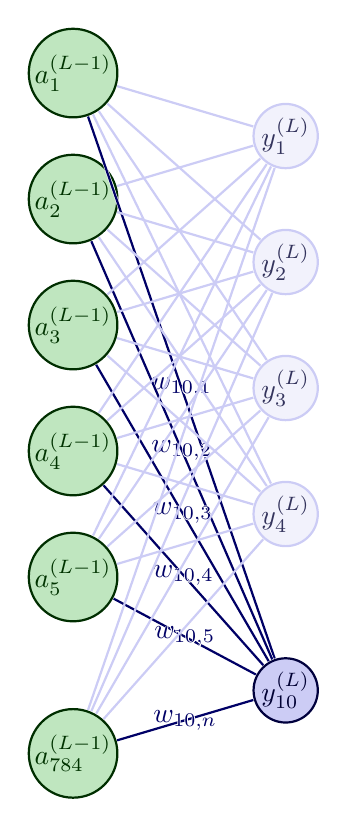
\begin{tikzpicture}[x=2.7cm,y=1.6cm]
  \message{^^JNeural network activation}
  \def\NI{6} % number of nodes in input layers
  \def\NO{5} % number of nodes in output layers
  
  \def\yshift{0.4} % shift last node for dots
  
  % INPUT LAYER
  \foreach \i [evaluate={\c=int(\i==\NI); \y=\NI/2-\i-\c*\yshift; \index=(\i<\NI?int(\i):"784");}]
              in {1,...,\NI}{ % loop over nodes
    \node[node in,outer sep=0.6] (NI-\i) at (0,\y) {$a_{\index}^{(L-1)}$};
  }
  
  % OUTPUT LAYER
  \foreach \i [evaluate={\c=int(\i==\NO); \y=\NO/2-\i-\c*\yshift; \index=(\i<\NO?int(\i):"10");}]
    in {\NO,...,1}{ % loop over nodes
    \ifnum\i=5 % high-lighted node
      \node[node hidden]
        (NO-\i) at (1,\y) {$y_{\index}^{(L)}$};
      \foreach \j [evaluate={\index=(\j<\NI?int(\j):"n");}] in {1,...,\NI}{ % loop over nodes in previous layer
        \draw[connect,white,line width=1.2] (NI-\j) -- (NO-\i);
        \draw[connect] (NI-\j) -- (NO-\i)
          node[pos=0.50] {\contour{white}{$w_{10,\index}$}};
      }
    \else % other light-colored nodes
      \node[node,blue!20!black!80,draw=myblue!20,fill=myblue!5]
        (NO-\i) at (1,\y) {$y_{\index}^{(L)}$};
      \foreach \j in {1,...,\NI}{ % loop over nodes in previous layer
        %\draw[connect,white,line width=1.2] (NI-\j) -- (NO-\i);
        \draw[connect,myblue!20] (NI-\j) -- (NO-\i);
      }
    \fi
  }
\end{tikzpicture}
\n
\caption{Random output of the example}
\label{NNHandwritingRanOut}
\end{figure}

\noindent Using methods to be discussed in Chapter \ref{developingNN}, we may adjust the weights and biases using different training data so that the ANN can classify with a higher accuracy. Eventually, the ANN may take a clear digit 7, and output results similar to table 1. As $i = 8$ is the brightest neuron, the network has selected 7 as the output. 
\end{example}
\newpage


\section{Activation Functions} \label{activationFunction}

As mentioned in section \ref{activation}, we use an activation function on $z$ to pass values forward through a network, rather than directly passing the value of $z$ through. It is natural to question why can't we directly feed through the value of $z$? Well, without an activation function, an ANN would behave like a linear regression model, performing linear transformations on the input, weights, and biases; there would be little need for multiple layers. This would reduce the accuracy in some cases, as the ANN could not be well trained for differing inputs. \\ 

Throughout this chapter, I will refer to $z$ as the input for the activation functions, as that is the case for this project. I advise the reader to be mindful that the calculation of $z$ initially may vary depending on the network. \\

As mentioned, in this project we use the sigmoid function, which is useful for classification problems. When adapting to different scenarios, however, different activation functions may be more appropriate. We shall explore some of the common types, including a deeper dive into the sigmoid function, next. 



\subsection{Binary Step Function} \label{BSF}
The Binary Step Function (BSF) works using a threshold \cite{BST}. If the input, $z$, meets a certain threshold, the neuron is activated. It is defined as follows: 

\begin{equation}
f(x) = \left\{
        \begin{array}{ll}
            1 & \quad x < 0 \\
            0 & \quad x \geq 0
        \end{array}
    \right.
\end{equation}
Due to the limited outputs (0 or 1), this is not useful for image classification. Suppose we had a network like example \ref{handwritingEG}. If we used the BSF, we may have multiple neurons in the output layer as 1. There would be no way for us to determine which neuron was the network's choice, as they would all have the same value of 1. \\

We will see later (section \ref{backPropagation}) that activation functions with a gradient of zero, like the BST, are not useful for the learning process.  

\subsection{Linear Activation Functions}
Linear Activation Functions (LAF) may be given by \cite{BST}: 
\begin{equation}
f(x) = x 
\end{equation}
Similarly to the BSF, LAFs are not useful for the learning process due to their gradient. The gradient is constant, does not vary with input, so cannot be used to adjust the weights and biases that we will see in section \ref{backPropagation}. \\ 

Using the LAF causes all preceding layers to become linear functions of the one before, making the use of layers somewhat redundant. As the use of layers is recommended in image recognition \cite{Java}, we do not use the LAF.  

\subsection{Non-Linear Activation Functions}
Unlike BSFs and LAFs, non-linear activation functions (NLAF) allow for system learning due to their non-constant gradient  (section \ref{backPropagation}). \\ 

There are many different NLAFs. I, however, shall highlight three of the most common NLAFs relevant to this project \cite{activationfunc}. 

\subsubsection{Sigmoid Function \label{sigmoid}}

We begin with the sigmoid function, equation \ref{sigmoidEqn}, which we use as follows : 
\begin{equation}
a^L = \sigma(z^L)  
\end{equation}

% I.e. $a^L ( w^L, a^{L-1}, b^L)$ 

Typically, the sigmoid function is used for probabilistic scenarios due to the output range $[0,1]$. In example \ref{handwritingEG}, we may think of the activation in the final layer as the probability that the number was the one that was fed into the network.  \\ 

Figure \ref{sigmoidgraph} shows $\sigma(x)$ and the gradient $\sigma '(x)$. You can see that the gradient is only significant for roughly $x \in [-3.5, 3.5]$. For values outside of this range, the gradient tends to 0, and the learning process may not be successful. This issue is referred to as the vanishing gradient problem. 

\begin{figure}[!b]
\centering
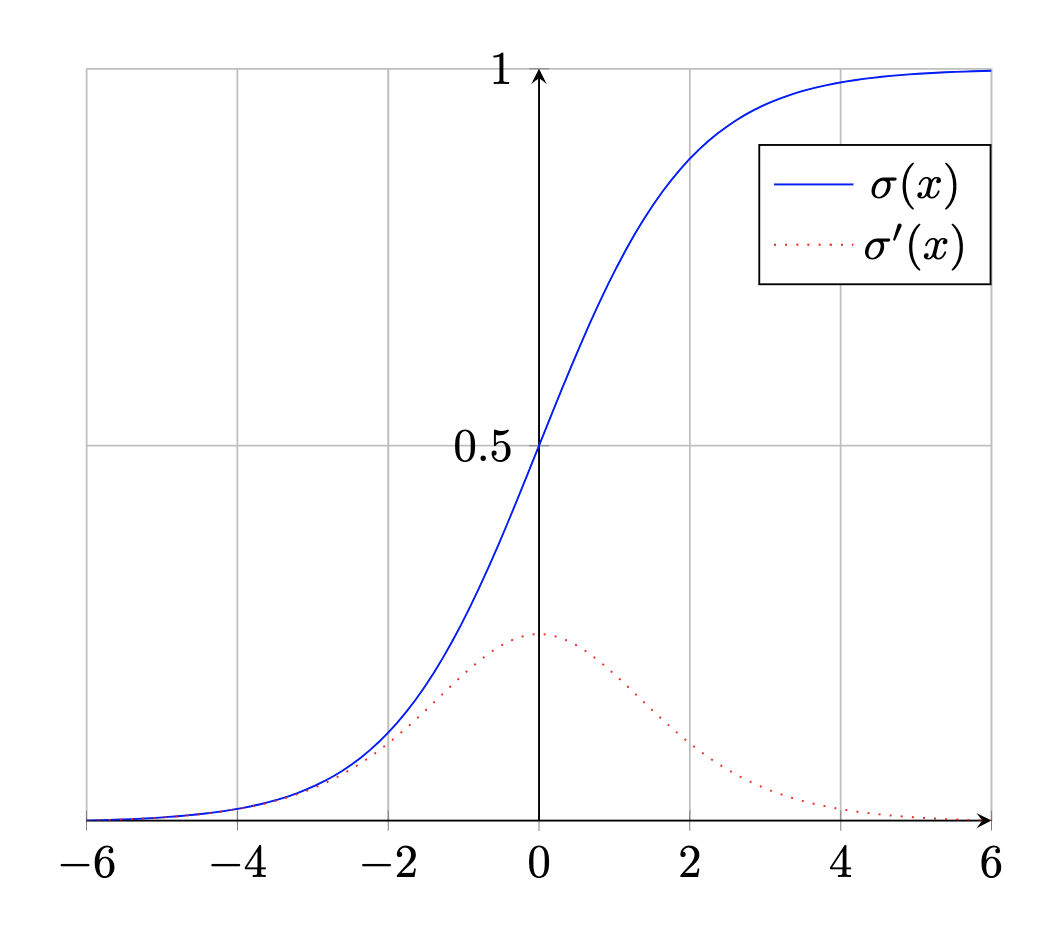
\includegraphics[width=12cm, height=10cm]{sigmoidgraph.png}
    \caption{Sigmoid Function and it's gradient}
    \label{sigmoidgraph}
\end{figure}


\subsubsection{Hyperbolic Tangent Function}
Another common activation function, $\tanh(x)$, gives a similar output to the sigmoid, and has a similarly behaving gradient. As a result, it too suffers from the vanishing gradient problem. \\ 

$\tanh(x)$, figure \ref{tanhgraph}, has outputs in the range $(-1, 1)$, and is defined as follows: 
\begin{equation}
\tanh(x) = \frac{e^{x} - e^{-x}}{e^{x}+e^{-x}}
\end{equation}
The hyperbolic tangent is more commonly used to indicate correlation. We want to see which neuron the network has classified, and thus only need positive values like the sigmoid function provides. Having positive and negative values may increase the difficulty of comparison for the brightest neuron. 
\begin{figure}[h!]
\centering
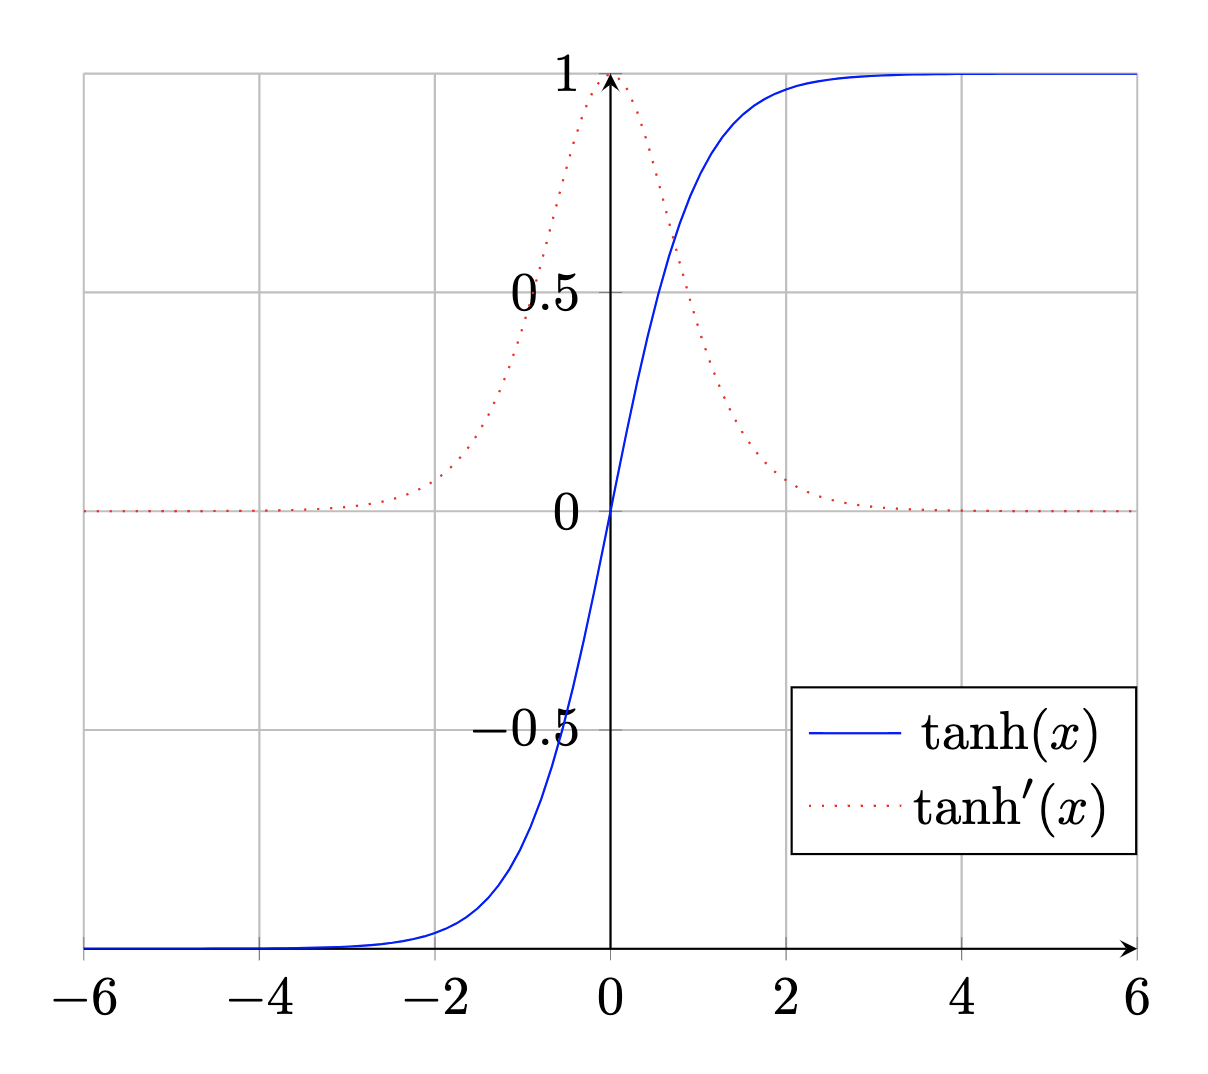
\includegraphics[width=12cm, height=10cm]{tanhgraph.png}
    \caption{Hyperbolic Tangent Function and it's gradient}
    \label{tanhgraph}
\end{figure}

\subsubsection{Rectified Linear Unit }

The Rectified Linear Unit (ReLU) is a non-linear activation function that behaves linearly \cite{relu}, defined as follows: 
\begin{equation} \label{relu}
f(x) = \text{max}(0,x)
\end{equation}
The ReLU function only activates neurons that end up with a positive activation value. If the input is less than 0, the function returns 0. It is commonly used for hidden layers to avoid the vanishing gradient problem. The derviative of the ReLU function is 0 for negative numbers, but 1 for positive inputs \cite{relu}. When using a large batch of training data, the average derivative is usually not zero, allowing for gradient descent. \\ 


Throughout this project we will use the sigmoid function as the restriction of outputs between [0,1] assists with visualising the learning process. However, it must be noted that due to the vanishing gradient problem, this is not always ideal. 

\newpage
\section{Learning in an ANN \label{developingNN}}
The first step of the learning process is to assess how incorrect, or correct, the network is by assessing the outputs,  $a_n^L = \sigma(z^L)$. We do this using the cost function. 


\begin{figure}[htp] \label{NNHandwriting_2layer}
\centering
% NEURAL NETWORK with coefficients, shifted
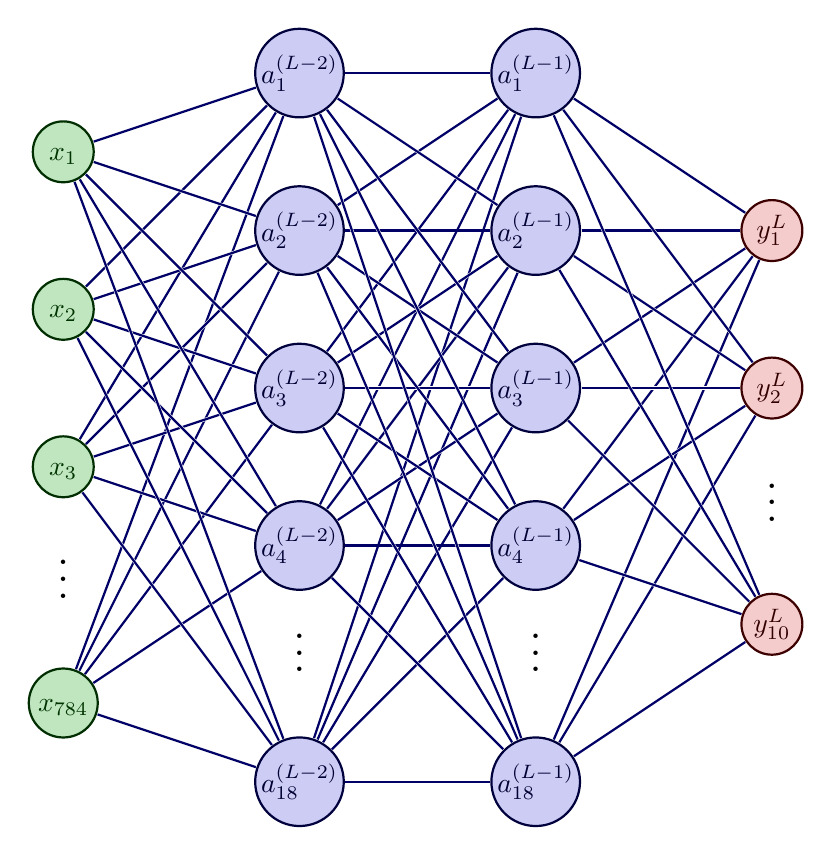
\begin{tikzpicture}[x=3cm,y=2cm]
  \message{^^JNeural network, shifted}
  \readlist\Nnod{4,5,5,3} % array of number of nodes per layer
  \readlist\Nstr{784,18,18,10} % array of string number of nodes per layer
  \readlist\Cstr{\strut x,a^{(L-2)},a^{(L-1)},y^{L}} %labels of neurons
  \def\yshift{0.5} % shift last node for dots
  
  \message{^^J  Layer}
  \foreachitem \N \in \Nnod{ % loop over layers
    \def\lay{\Ncnt} % alias of index of current layer
    \pgfmathsetmacro\prev{int(\Ncnt-1)} % number of previous layer
    \message{\lay,}
    \foreach \i [evaluate={\c=int(\i==\N); \y=\N/2-\i-\c*\yshift;
                 \index=(\i<\N?int(\i):"\Nstr[\lay]");
                 \x=\lay; \n=\nstyle;}] in {1,...,\N}{ % loop over nodes
      % NODES
      \node[node \n] (N\lay-\i) at (\x,\y) {$\Cstr[\lay]_{\index}$};
      
      % CONNECTIONS
      \ifnum\lay>1 % connect to previous layer
        \foreach \j in {1,...,\Nnod[\prev]}{ % loop over nodes in previous layer
          \draw[connect,white,line width=1.2] (N\prev-\j) -- (N\lay-\i);
          \draw[connect] (N\prev-\j) -- (N\lay-\i);
          %\draw[connect] (N\prev-\j.0) -- (N\lay-\i.180); % connect to left
        }
      \fi % else: nothing to connect first layer
      
    }
    \path (N\lay-\N) --++ (0,1+\yshift) node[midway,scale=1.5] {$\vdots$};
  }
  
  % LABELS
%  \node[above=5,align=center,mygreen!60!black] at (N1-1.90) {input\\[-0.2em]layer};
 % \node[above=2,align=center,myblue!60!black] at (N3-1.90) {hidden layers};
  %\node[above=10,align=center,myred!60!black] at (N\Nnodlen-1.90) {output\\[-0.2em]layer};
  
\end{tikzpicture}
\caption{ANN for handwriting recognition of 28 x 28 pixel image}
\end{figure}



\subsection{Cost Function}
\label{CostFunction} 
To determine the cost of the network, first we look at the loss of the network. We define the loss as the square of the difference between the actual output, $t$, and the expected output, $y$. 
\begin{equation} 
(y-t)^2
\end{equation}

\noindent We then form the mean-squared error cost function: 
\begin{equation} \label{costfunction}
C =\frac{1}{n} \sum_{i=1}^{n} (y-t)_i ^2 
\end{equation}
%https://towardsdatascience.com/machine-learning-fundamentals-via-linear-regression-41a5d11f5220

%Perhaps explore additional cost functions and their effects 
%MAYBE RE-DO THIS EQN WITH aL etc. 
%ALSO NOTE that under grad desc. we use C= 1/n sum etc. 

Where i = index of neuron, $y$ denotes the desired output, and $t$ denotes the actual output (i.e. $t_i = a_i^L$). \\ 


The cost of a network, $C$,  is a $k$-dimensional column vector, where $k$ is the number of output neurons. 

\begin{example} \label{cost_function_eg} 
Building on example \ref{handwritingEG}, table 1, we assess the cost function using $t^L_i$ and $y^L_i$  (table 3):   \\  
\begin{minipage}[c]{0.5\textwidth}
\begin{center}
\begin{tabular}{ |c |c |c|}
\hline
 $i$ &  $t_i^L$ & $y_i^L$\\
\hline
 1 & 0.03  & 0.00\\ 
  2 & 0.02 & 0.00 \\  
  3 & 0.08  & 0.00 \\
   4 & 0.34 & 0.00  \\ 
  5 & 0.56  & 0.00\\  
   6 & 0.58  & 1.00\\ 
  7 & 0.12  & 0.00\\  
   8 & 0.39  & 0.00\\ 
  9 & 0.60  & 0.00\\  
   10 & 0.97 & 0.00  \\
   \hline
   \end{tabular}
\captionof{table}{\\Table 1 with the desired outputs, y}
\label{table1EGH_y}
\end{center}
\end{minipage}
\begin{minipage}[c]{0.5\textwidth}

Using equation \ref{costfunction}: 
\newline 
$C = (0.03 - 0.00)^2 + (0.02 - 0.00)^2 + (0.08 - 0.00)^2 + (0.34 -0.00)^2 + (0.56 - 0.00)^2 + (0.58 - 1.00)^2 + (0.12 - 0.00)^2 + (0.39 - 0.00)^2 + (0.60 - 1.00)^2 + (0.97 - 1.00)^2  $ 
\\
\newline 
$C = 2.0807 $ 
\end{minipage}
\end{example} \\
\newpage
\subsubsection{What does the cost function tell us?} 
The smaller the cost function, the better the performance of the ANN. A small value indicates that the difference between the actual and desired output is small, and thus the network is correctly classifying. The exact value depends upon the network and goals. The last example, example \ref{cost_function_eg}, depicts an unsuccessful network. 

\subsubsection{Using a Cost Function to develop an ANN}
As we want our $C$ to have the smallest possible value, we aim to minimise it. To do this, first we first allocate random weights and biases; this will likely cause random and very incorrect outputs (as in example \ref{handwritingEG}). Then, we run the network with a random piece of data from the training set, and evaluate the cost. We then use gradient descent, discussed in section \ref{gradient descent}, to determine how to minimise the cost, make those changes, and start again with a new piece of training data. This is called the learning phase.  \\ 

%We could randomly change the weights and biases throughout, but when we're working with a network such as the demonstrated in example \ref{handwritingEG} (handwriting example), with thousands of weights and biases, this is not feasible. 

\subsection{Gradient Descent \label{gradient descent}}
In section \ref{structure} we introduced the structure of an ANN. Considering this along with the equation for $C$, equation \ref{costfunction}, we see that to minimise the cost, we need any of the following to change \cite{Marsland}: 
\begin{enumerate}
\item The inputs $x_1, x_2, ..., x_n$ 
\item The activations 
\item The weights and biases 
\end{enumerate}
 \\

We cannot change the inputs, nor can we directly change the activations (as they are a function of the input and weights). We can, however, change the weights and biases, which then adjusts the activations; this process is gradient descent. 
\\ 
% https://latexdraw.com/three-dimensional-plotting-in-latex/ 

The positive gradient of the cost function, $\bigtriangledown C$,  tells us which direction to move in to increase the function the quickest. Therefore, if we take the negative gradient, we can determine how to minimise the function. 
\begin{equation} \label{deltaC}
\bigtriangledown C = \begin{bmatrix}
\frac{\partial C}{\partial w^1}\\
\frac{\partial C}{\partial b^1} \\ ... \\ \frac{\partial C}{\partial w^L} \\ \frac{\partial C}{\partial b^L}
\end{bmatrix}
\end{equation}
\\ 
Then we may adjust the weights as follows: $w'^L_{ji} = w_{ji} ^L - \frac{\partial C_k}{\partial w^L_{ji}}$, and similarly for the biases. We will explore how to calculate these in section \ref{backPropagation}.  \\ 

An issue with gradient descent is that we may locate only a local minimum, rather than a global. To overcome this, we adapt our method of gradient descent. The process we use in this project is Stochastic Gradient Descent (SGD), updating the weights and biases with each iteraction of the ANN. SGD suffers from noise issues, but helps minimise the local minima issue \cite{DeepPy}. 



\begin{example}
Take this random list of all weights and biases: \\
\begin{center}
$ \overrightarrow{w} =  \begin{bmatrix}
2.25\\-1.57 \\ 1.98 \\ ... \\ -1.16 \\ 3.82 \\ 1.21 

\end{bmatrix} $
\end{center}

Using methods to be discussed, we may determine the negative gradient, $- \bigtriangledown C$, to see how to adjust each of the above to minimise the cost. Propose we have the following result for $- \bigtriangledown C$: 
\begin{center}
$- \bigtriangledown C( \overrightarrow{w}) = \begin{bmatrix}
-0.18\\0.45 \\ -.051 \\ ... \\ 0.40 \\ -0.32 \\ 0.82
\end{bmatrix} $
\end{center}
This tells us that we may make the following changes to the ANN: \\ 
$w_1 +0.18, w_2 - 0.45, w_3 +0.051$, ..., $w_{n-2} - 0.40, w_{n-1} + 0.32, w_n - 0.82$ 
\end{example}

Making the direct changes $w'^L_{ji} = w_{ji} ^L - \frac{\partial C_k}{\partial w^L_{ji}}$ can alter the network too drastically, damaging the learning process. To overcome this issue, we introduce the learning rate, $\eta $. 



\subsubsection{Learning Rate}
The learning rate is a positive parameter $\eta$ used to stabilise the ANN throughout the learning process by determining the rate at which the ANN learns \cite{Marsland}. Without it, the network would change significantly with each incorrectly classified image. This could cause instability and fluctuation and lead to the cost function not reducing. It is used as follows: 

\begin{equation} \label{lreqn}
\Delta w =-\eta \bigtriangledown C
\end{equation}
Meaning each weight is adjusted according to: 

\begin{equation} 
w'^L _{ji} =w^L _{ji} -\eta \frac{\partial C_k }{\partial w^L_{ji}} 
\end{equation}
\textbf{Values of $\eta$}

The value of $\eta$ varies depending on the network. Typical values of $\eta$ are within the range $[0.1, 0.4]$, \cite{Marsland}. Setting $\eta = 1$  is the equivalent of not using it (see equation \ref{lreqn}). The smaller the value, the longer the ANN may take to learn. In practice, we should adjust the value of $\eta$ throughout the learning process, using a larger $\eta$ initially to increase the speed of the learning process. When the cost function noticeably reduces and the weights and biases settle, we reduce the learning rate to prevent drastic changes. 
\\ 
 % http://neuralnetworksanddeeplearning.com/chap1.html#the_architecture_of_neural_networks
%sort out indices etc. 

\subsubsection{Stochastic Gradient Descent with Backpropagation} \label{backPropagation}

Backpropagation is a form of gradient descent where we work backwards through the ANN to evaluate errors and make adjustments \cite{Marsland}. Back-propagation enables us to find $ \bigtriangledown C$, recall equation \ref{deltaC}, for the entire network, i.e. $\frac{\partial C }{\partial w}$. In this subsection we will look at the calculation of these derivatives. We will set the foundations with the weights, and we can then translate equations easily for biases. \\ 

%Take this NN: 
% PICTURE FROM PG23 OF NOTES  (each layer has one neuron) 

To begin the calculations, lets consider a simple ANN with four layers, and one neuron in each, as shown in figure \ref{singleANN}.  

% cannot get the nodes to update to be values %adjust the following to look less weird 
\begin{figure}[h!] 
\centering
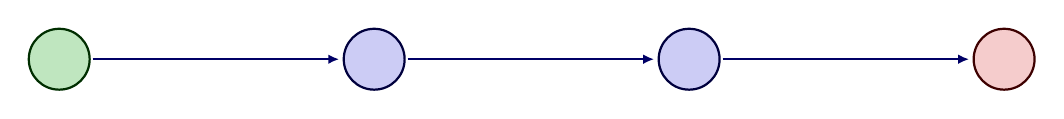
\begin{tikzpicture}[x=4cm,y=1cm]
  \message{^^JNeural network with arrows}
  \readlist\Nnod{1,1,1,1} % array of number of nodes per layer
  
  \message{^^J  Layer}
  \foreachitem \N \in \Nnod{ % loop over layers
    \edef\lay{\Ncnt} % alias of index of current layer
    \message{\lay,}
    \pgfmathsetmacro\prev{int(\Ncnt-1)} % number of previous layer
    \foreach \i [evaluate={\y=\N/2-\i; \x=\lay; \n=\nstyle;}] in {1,...,\N}{ % loop over nodes
      
      % NODES
      \node[node \n] (N\lay-\i) at (\x,\y) {};
      %\node[circle,inner sep=2] (N\lay-\i') at (\x-0.15,\y) {}; % shifted node
      %\draw[node] (N\lay-\i) circle (\R);
      
      % CONNECTIONS
      \ifnum\lay>1 % connect to previous layer
        \foreach \j in {1,...,\Nnod[\prev]}{ % loop over nodes in previous layer
          \draw[connect arrow] (N\prev-\j) -- (N\lay-\i); % connect arrows directly
          %\draw[connect arrow] (N\prev-\j) -- (N\lay-\i'); % connect arrows to shifted node
        }
      \fi % else: nothing to connect first layer
      }
   }
  \end{tikzpicture}
\caption{Single Layer Network}
\label{singleANN}
\end{figure}
%below - see pg 60/61 of logbook 
\\ 
$C$ is a function of $a^L, w^L, a^{L-1},$ and $b^L$ , i.e.: $C(a^L, w^L, a^{L-1}, b^L)$. By the chain rule:
\begin{equation} \label{costpartials}
\frac{\partial C_k}{\partial w^L} = \frac{\partial z^L}{\partial w^L} \frac{\partial a^L}{\partial z^L} \frac{\partial C_0}{\partial a^L}
\end{equation}

Where $k$ refers to the piece of training data. Using the definitions of $a^L$, $z^L$, $C_k$ (see section  \ref{provingdc/dw} in the appendices), we see that 
\begin{equation} \label{dc/dw}
 \frac{\partial C_k}{\partial w^L} = 2a^{L-1}   (a^L - y)   \sigma ' (z^L)
\end{equation}

Equation \ref{dc/dw} tells us how a change to a particular weight, $w_L$, will affect the cost for the $k$th training example. To calculate the cost for all of the training data, $C$, we calculate the average of all costs from the training data using equation \ref{costfunction}\cite{NN}. That is, from k = 1 to k = n. 
\begin{equation}
\frac{\partial C}{\partial w^L} = \frac{1}{n}   \sum_{k=1}^{n} \frac{\partial C_k}{\partial w_L}
\end{equation}
Calculating $\frac{\partial C_k}{\partial b^L}$ uses the same process and has a similar result. However, as $\frac{\partial z^L}{\partial b^L} = 1$: 
\begin{equation} \label{biasdif}
\bigtriangledown C = \frac{\partial a^L}{\partial b^L} \frac{\partial C_0}{\partial a^L}
\end{equation}
 \\ 

So far, we have only focussed on the output layer. Consider figure \ref{treeDiag}, showing the relationship between $C$ and different layers of the ANN in \ref{singleANN}. We see that $C$ is influenced by all elements of the network, but less so as we go further back through the network (that is, from the output, $L$, to earlier layers, say $L-2$). We deduce that $w^L$ has more influence on C than $w^{L-1}$ . 

\begin{figure}[h!]
\centering
\begin{tikzpicture}
  [
    grow                    = left,
    sibling distance        = 3em,
    level distance          = 5em,
    edge from parent/.style = {draw, -latex},
    every node/.style       = {font=\footnotesize},
    sloped
  ]
  \node [dummy] {$C_0$}
    child { node [dummy, size=2cm] {$y$}
      edge from parent node [below] {} }
    child { node [dummy, size=6cm] {$a^L$}
      child { node [dummy] {$z^L$}
        child { node [dummy] {$w^L$}
          edge from parent node [below] {} }
        child { node [dummy] {$a^{L-1}$}
             child { node [dummy] {$...$}}
          edge from parent node [above] {}
                           node [below] {} }
        child { node [dummy] {$b^L$}
                edge from parent node [above] {} }
        edge from parent node [below] {} }
      };
\end{tikzpicture}
\caption{}
\label{treeDiag}
\end{figure}

We cannot use the same derivative, equation \ref{dc/dw}, for elements in the hidden, or input, layers. However, similar to equation \ref{costpartials}, we can use the chain rule to obtain: 
\begin{equation}
\frac{\partial C_k}{\partial w^{L-1}} = \frac{\partial z^{L-1}}{\partial w^{L-1}} \frac{\partial a^{L-1}}{\partial z^{L-1}}\frac{\partial {z^L}}{\partial a^{L-1}}  \frac{\partial a^{L}}{\partial z^{L}}\frac{\partial C_0}{\partial a^L}
\end{equation}
Now that we can calculate $\bigtriangledown C$ for a network with one neuron in each layer, it is easy to translate this to a multilayer network with one or more neurons in each. Using equation \ref{costpartials}, we determine: 
\begin{equation}
\frac{\partial C_k}{\partial w^L_{jk}} = \frac{\partial z_j^L}{\partial w_{jk}^L} \frac{\partial a_j^L}{\partial z_j^L} \frac{\partial C_0}{\partial a_j^L}
\end{equation}

In section \ref{coding_nn}, I will demonstrate briefly my coding of an ANN using backpropagation. 


\newpage

\section{ANN: Coding a Neural Network} \label{coding_nn}

% Use one hidden layer - will help with back prop. See nielsen book for info 
%This resource might be helpful: https://arxiv.org/pdf/1805.09190v3.pdf 
% Using Python or C++ 

It is common that the processes discussed in this report will be performed by a machine as, unless the network consists of a handful of components, it is not feasible to compute by hand. Common coding languages to use include Python, C++, and Java \cite{Java}. I have chosen C++ due to it's higher performance power. 

\subsection{Perceptron Network}

Using the simple network modelled in section \ref{Perceptron}, I created a piece of code in C++ to model this and perform the learning process. You may find the code in \ref{simpleNN}, and figure \ref{flowchart} shows a diagram of the processes. \\

The learning process of this code involves backpropagation using equation \ref{dc/dw}, where only layers $L$ and $L-1$ are considered. This was a simple network, but effective to build upon for multilayer networks. The code was successful in the learning process, as confirmed by my supervisor. 


\subsection{Multilayer Network}
\textit{This refers to the code in the appendices: section \ref{pixelValCode}. }\\

Next, I created a code that accounts for multiple layers. This code has four inputs, $A,B,C,D$ and two outputs $W,B$. The four inputs represent a $4$ x $4$ pixel image, with grayscale values. Using an average rule, the network decides whether the image was mostly black pixels, or mostly white. \\

Once this network is established, the reader may develop the code to structure the network to suit their needs. Future studies for myself would include a code whose core learning component is not restricted to a certain amount of neurons - in this case 4 outputs. \\

A $k$-dimensional vector is created to store all weights, and $m$-dimensional to store all biases, where $k$ and $m$ are the amount of weights and biases in the network respectively. Random weights in the range 0 to 9 are then assigned. At first, this range was larger - but the network was not reducing the cost. Upon research \cite{weightvals}, I found that the amount of weights is typically in the range $[-1,1]$, but can vary. I had little variation in the outputs when adjusting the initial random weight range between [-1, 1] and [0,9]. I have left the weight range as [0,9] for now, however, this may be changed by the reader as necessary. \\

Weights and biases are kept in separate vectors for the code as, although the learning process is the same, the equations for backpropagation vary - see equation \ref{biasdif}. \\

The code works using a loop which restricts the amount of iterations, again set by the user manually.\\

Within the loop, the random grayscale values of the inputs are assigned. I created the following rule for the outputs: 

\begin{equation}
\frac{A + B + C + D}{4} > 0.5 \implies \text{output black}
\end{equation}\begin{equation}
\frac{A + B + C + D}{4} \leq 0.5 \implies \text{output white}
\end{equation}The network then runs the randomly assigned values using the sigmoid function, equation \ref{sigmoidEqn} and random weights and biases. \\

Afterwards, the contents of the loop move on to gradient descent, following the steps laid out to the reader in section \ref{backPropagation}.  New vectors of $k$ and $m$ dimensions respectively are created to hold the values of $\bigtriangledown C$. The expected outputs, $y$ are assessed using the rule above. Rather than perform differentiation directly in the code, we develop relations specifically for this network, as you will see in the appendices, section \ref{pixelValCode}\\ 

The final step of the loop is to implement the changes to the weights and biases using the respective $\bigtriangledown C$ vectors. These weights and biases are used for the next iteration with again random grayscale values. \\

In future studies, I would require my code to pull data directly from data sets, and learn from these. \\

The results of my code show improvements in the network, however the cost function does not significantly reduce, even with millions of iterations. Given more time, we would explore this. However, for now it is apparent that my network's process of gradient descent is not successful for the required purpose. \\

The topic of neural networks and developing them becomes a topic of computer science, rather than mathematics. So, we shall begin looking at other methods of image recognition shortly. Prior to this, we shall visit some types of neural network and how they may impact the process. 
\begin{figure}[h!]
\begin{center}
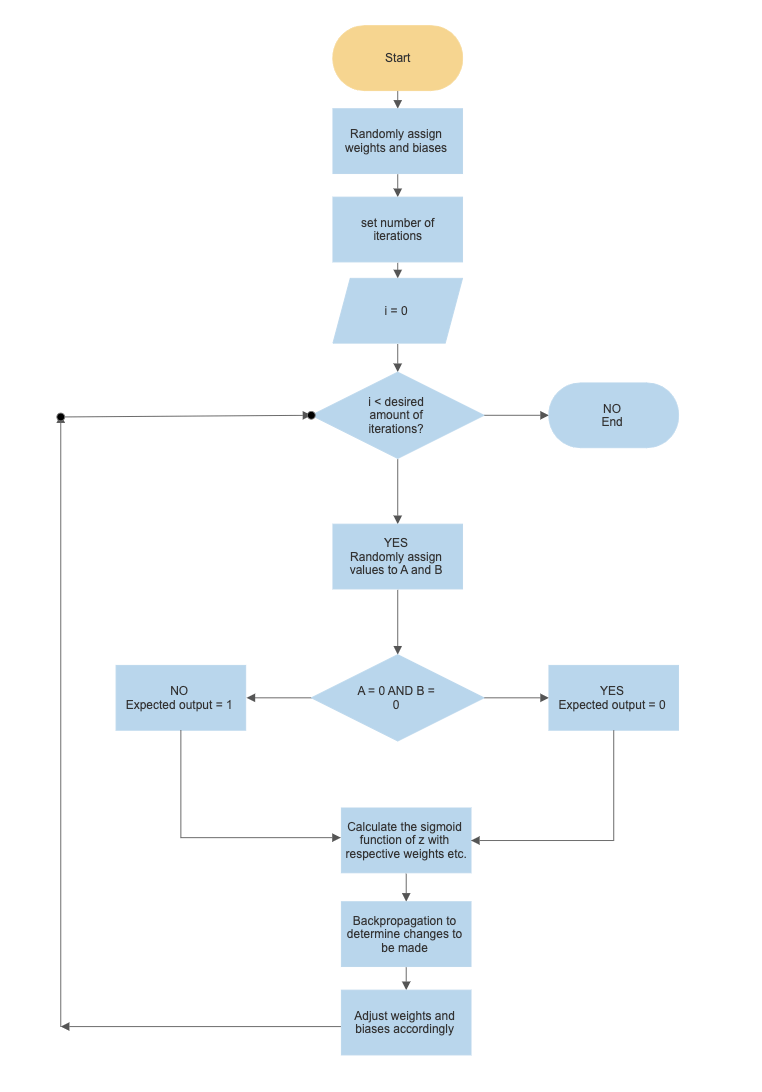
\includegraphics[width=\textwidth,height=\textheight,keepaspectratio]{Flowchart.png}
   \caption{Process of the Perceptron Code}
   \label{flowchart}
\end{center}
\end{figure}
\NEWPAGE

\newpage
\section{Types of Neural Network }
% Learning, RNN % https://en.wikipedia.org/wiki/Recurrent_neural_network 
\label{types}
Before moving on to handwriting recognition methods beyond neural networks, I shall introduce and compare some types of neural networks and how they may play a role in image recognition. 

\subsubsection{ANNs }
\label{ANN} So far we have considered ANNs; these feed data forward through the network. They have common uses in basic image recognition such as handwritten digits \cite{typesNN}. They are universally used, primarily for their use of activation functions, and ability to map non-linear functions with the use of weights and biases.  \\

ANNs have restrictions though, such as the input being 1-dimensional. For example, the images we have looked at throughout have been split into a 1-dimensional vector with 784 inputs. This restricts the learning process, as the ANN can only train on the one parameter. Additionally, spacial features (such as the placement of pixels), are lost within an ANN. For image classification, this is not too vital. However, if we required our network to tell us the positioning of particular pixels, or wanted it to classify depending upon the positioning of pixels, it could not. 

\subsubsection{RNNs}
Another type of neural networks is a recurrent neural networks (RNN), commonly used in audio and text. Within the hidden layers, data loops back to neurons, capturing sequential data \cite{RNN}; something ANNs cannot do. For example, the dependency on certain words when using predictive text is sequential data. The issue of digit recognition from a set of independent data would not require this. However, it may be used if this project was taken further to recognise words from handwriting samples. 

\subsubsection{CNNs}
The next type to mention are convolutional neural networks (CNN). CNNs use kernels (filters) to extract features, and are more commonly used for sophisticated image processing, considering images of objects with RGB colour values rather than grayscale. For example, you may input an image of an animal, and the CNN could classify whether it was a cat or not. CNNs can be used for handwriting recognition\cite{CNNHandwriting}, but for the purpose of a mathematical report I do not explore this. 

\subsection{Types of Learning}
It is also important to identify the types of learning. Throughout, we have used supervised learning. \cite{Marsland}. \textbf{Supervised} learning is where the network is provided with examples of correct outputs (our training set), so it can learn where it goes wrong and generalise responding. \\ 

On the other hand, we have \textbf{unsupervised} learning, where networks are not provided with correct examples. Rather, the networks find patterns so that certain inputs can be categorised. For example, an unsupervised digit recognition network may categorise images with certain average heights, or widths. This approach is sometimes called density estimation. \\

There is a mix between supervised and unsupervised, that is \textbf{reinforced} learning. The network is told when it is wrong, but not how to improve. The network then tries different possibilities until it reaches a correct answer. \\

\subsection{Generating Images using Neural Networks}

In subsection \ref{ANN}, we discussed a restriction of ANNs - they cannot capture spacial features. There are other types of neural networks that can, and we may use these to assess what makes up the average digit, and reconstruct images. In the world of computer science, there are two main networks to perform this process: autoencoders, and generative adversarial networks (GANs). GANs are a type of CNN \cite{GAN}. Autoencoders focus on decoding and encoding a network. Or, in our case, classifying digits, and recreating them. GANs on the other hand are focussed more on regenerating data, and classifying images as real, or re-generated. As we are focussing on recognition and processing, we shall explore autoencoders. 

\subsubsection{Autoencoders }
\label{Autoenc} Autoencoders are a form of unsupervised neural network that works to reconstruct data to represent the original data \cite{autoenc}. Autoencoders are commonly used for de-noising, but have been used to generate handwritten digits after training on a data set such as the MNIST \cite{MNIST}, such as figure \ref{reconstruct6} reconstructed from figure \ref{original6}. You will see that the reconstructed images are themselves noisy, and may not be clear to use, for example when making a font. In section \ref{Sobel}, we will see a method of edge detection filtering that enhances such images. Should this project be revisited, we may use autoencoders directly, and compare their outputs with GANs.  \\ 

Autoencoders are more complicated Neural Networks than the ones discussed earlier in the report, for example figure \ref{basicANN}. Their basic structure is similar however, shown in figure \ref{AutoEncStructure}, consisting of an input and output layer, and layers in between that are structured like a bottleneck \cite{autoenc}. Loss functions are used here too, ranging from the mean squared error which we have seen, to Kulback-Leibler Divergence (KLD) \cite{DKL} for variational autoencoders. \\ 

The KLD compares two probabilistic distributions, and may be used to compare actual outputs, $t_L$, to the desired output, $y_L$. For two discrete distributions, $P$ and $Q$, the KLD between them is given by: 
\begin{equation}
D_{KL}(P||Q) = \Sigma _x P(x) log \frac{(P(x))}{(Q(x))}
\end{equation}


\begin{figure}[!h!]
  \centering
  \begin{minipage}[b]{0.4\textwidth}
    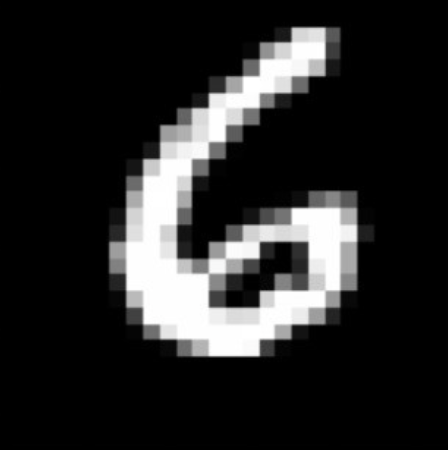
\includegraphics[width=\textwidth]{original6.png}
    \caption{Original}
    \label{original6}

  \end{minipage}
  \hfill
  \begin{minipage}[b]{0.4\textwidth}
    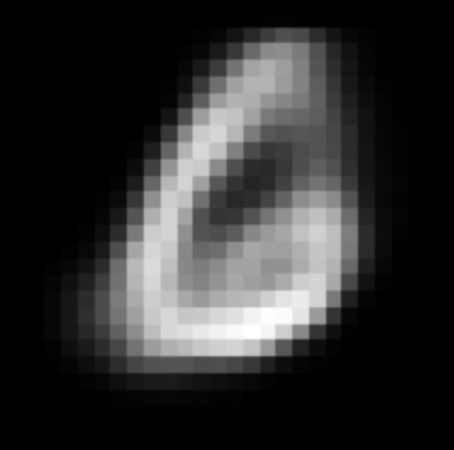
\includegraphics[width=\textwidth]{reconstruct6.png}
    \caption{Reconstructed}
    \label{reconstruct6}
  \end{minipage}
\end{figure}

%ANYMORE? BUILD ON THIS 

\begin{figure}[!h]
\centering
\begin{neuralnetwork}[height=8]
  \tikzstyle{input neuron}=[neuron, fill=mygreen!60!];
  \tikzstyle{output neuron}=[neuron, fill=myred!60!, text=white];

  \inputlayer[count=8, bias=false, title=Input]

  \hiddenlayer[count=5, bias=false]
  \linklayers

  \hiddenlayer[count=3, bias=false]
  \linklayers

  \hiddenlayer[count=5, bias=false]
  \linklayers

  \outputlayer[count=8, title=Output]
  \linklayers

\end{neuralnetwork}
\caption{Autoencoder Structure}
\label{AutoEncStructure}
\end{figure}
\newpage




\newpage

\section{Edge Detection Filters}
\label{Sobel} So far we have considered using ANNs to identify and classify handwritten digits. However, in my research plan (see appendices, \ref{researchP}) I laid out my motivation for researching image recognition. This was that, in year two of my degree, I produced a research poster on the Sobel Filter\cite{SobelFilter}, section \ref{SobelPoster} in the appendices, an edge detection filter (EDF). Though I have deviated from this process, I want to touch upon such methods, as they may be used with neural networks, such as autoencoders, to refine and enhance images and outputs. \\ 

EDFs detect boundaries with significant differences in brightness, typically using grayscale. For example, figure \ref{edgeexample} \cite{EdgeDetecImage}, which uses the canny edge detection algorithm. I propose the use of edge detection filters on the outputs of autoencoders, section \ref{Autoenc}, to refine images. The outputs may then be used, for example to create a font. 

\begin{figure}
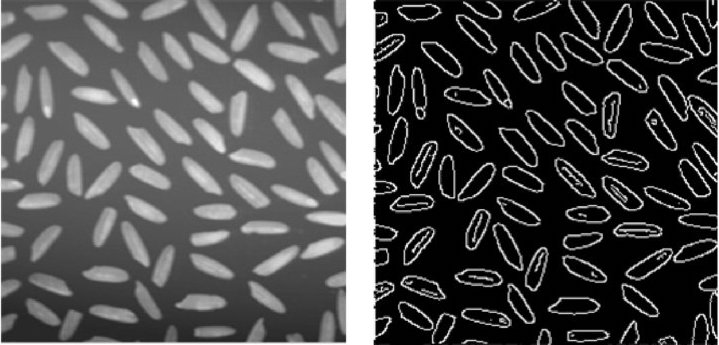
\includegraphics[width=\textwidth]{randEdgeDetec.jpeg}
    \caption{Edge Detection Example}
    \label{edgeexample}
\end{figure}

% https://www.researchgate.net/profile/Djemel-Ziou/publication/312890367_'Edge_detection_techniques_An_overview'/links/59d3c61c0f7e9b4fd7ffbfbb/Edge-detection-techniques-An-overview.pdf

\subsubsection{The Sobel Filter}
The Sobel Filter, or the Sobel–Feldman Operator (SFO), uses gradient filters to refine images \cite{sobel}. It builds upon earlier work estimating the gradient vector using the following masks \cite{edgePDF}: \\ 

\begin{minipage}[c]{5cm}
\begin{equation}
\bigtriangleup _x = 
\begin{bmatrix}
-1 & 0 & 1\\
-a & 0 & a \\ 
-1 & 0 & 1 
\end{bmatrix}
\end{equation}\end{minipage}
\begin{minipage}[c]{5cm}
\centering
and 
\end{minipage}
\begin{minipage}[c]{5cm}
\begin{equation}
\bigtriangleup _y = 
\begin{bmatrix}
-1 & a & -1\\
0 & 0 & 0 \\ 
1 & a & 1 
\end{bmatrix}
\end{equation}\end{minipage}
where $a > 0, a\in \mathbb{R}$

The SFO uses $a = 2$, i.e. the two $3$x$3$ kernels: \\ 
\begin{minipage}[c]{5cm}
\centering
\begin{equation}
\bigtriangleup _x = 
\begin{bmatrix}
-1 & 0 & 1\\
-2 & 0 & 2 \\ 
-1 & 0 & 1 
\end{bmatrix}
\end{equation}\end{minipage}
\begin{minipage}[c]{5cm}
\centering
and 
\end{minipage}
\begin{minipage}[c]{5cm}
\centering
\begin{equation}
\bigtriangleup _y = 
\begin{bmatrix}
-1 & 2 & -1\\
0 & 0 & 0 \\ 
1 & 2 & 1 
\end{bmatrix}
\end{equation}\end{minipage}

We then use the kernels on the source image $\textbf{A}$ as follows: 
\begin{equation} \label{usingSobel}
G_x = X * A , \\ 
G_y = Y * A 
\end{equation}
where $*$ is the convolution operation. \\

The result of equation \ref{usingSobel} describes the differentiation in grayscale values between pixels. A larger values means a more noticeable edge due to greater differences in value. Performing equation \ref{usingSobel} on the entire image allows us to replace the previous grayscale values with the result. For example, the SFO applied to figure \ref{reconstruct6} returns figure \ref{SFfigure}. Although figure \ref{SFfigure} is noticeably clearer than figure \ref{reconstruct6}, it still has noise. To overcome this, we may us an averaging filter prior to the SFO\cite{sobelIs}.  \\ 
%build on?  \\ 


In figures \ref{RCfigure} and \ref{Lfigure}, you see the results of two other EDFs that perform, and produce outputs, similar to the SFO. The Robert Cross EDF uses two $2$x$2$ kernels, and the Laplacian uses a $3$x$3$ mask. Future work on this project may include the comparison of such methods on the results of an Auto Encoder. 

% Identifies 'differentiation' - large changes in values, e.g. grayscale here - to produce 'outlines'.  %https://www.researchgate.net/profile/Djemel-Ziou/publication/312890367_'Edge_detection_techniques_An_overview'/links/59d3c61c0f7e9b4fd7ffbfbb/Edge-detection-techniques-An-overview.pdf 


\begin{figure}[!h!]
  \centering
   \begin{minipage}[b]{0.4\textwidth}
    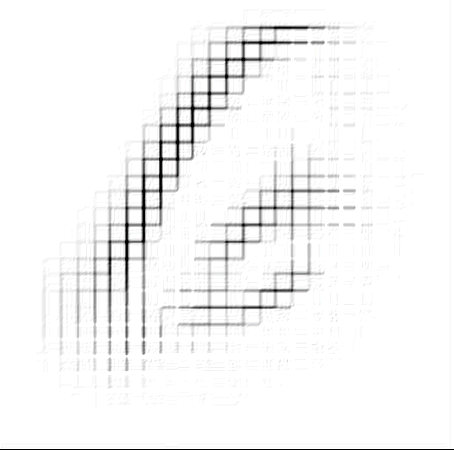
\includegraphics[width=\textwidth]{rc6.png}
    \caption{Figure \ref{reconstruct6} reconstructed using Roberts Cross EDF \cite{onlinefilters}}
    \label{RCfigure}
  \end{minipage}
  \hfill
  \begin{minipage}[b]{0.4\textwidth}
    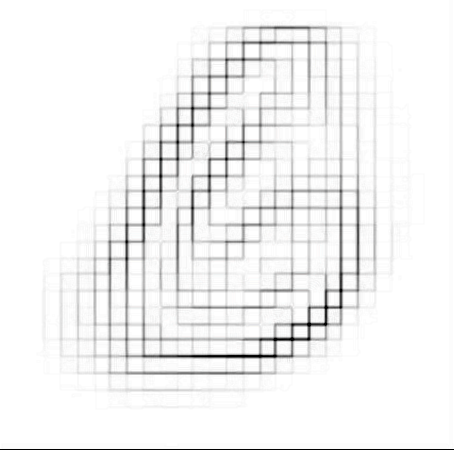
\includegraphics[width=\textwidth]{sf6.png}
    \caption{Figure \ref{reconstruct6} reconstructed using Sobel Feldman EDF \cite{onlinefilters}}
    \label{SFfigure}
  \end{minipage}
  \hfill
    \begin{minipage}[b]{0.4\textwidth}
    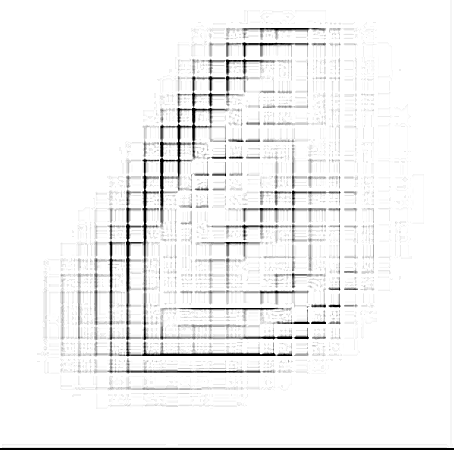
\includegraphics[width=\textwidth]{l6.png}
    \caption{Figure \ref{reconstruct6} reconstructed using Laplacian EDF \cite{onlinefilters}}
    \label{Lfigure}
  \end{minipage}
  
\end{figure}
\newpage

\section{Interpolation} \label{interpolation} 
% https://towardsdatascience.com/polynomial-interpolation-3463ea4b63dd
 In this chapter, we explore how polynomial interpolation may be used for image recognition. Interpolation provides a means of estimating the function at intermediate points. \\ 
 
 %We will assess the suitability of each method to estimate functions, in this case plots of digits or characters. 
 
%\textbf{Before we move on, it is imperative to mention other methods, such as nearest neighbour decoding... }

To begin, we may consider handwritten digits as graphs. Treating the interface as an axis, we can take the coordinates of points along the ink trace. For example, in figure \ref{abnodots} we have two handwritten characters. Figure \ref{abdots} shows how we may record the coordinates, with the yellow dots showing the trace, and the red dots showing where the pen starts touching the interface, and where it stops. \\
\\ 
In this section we explore methods using the coordinates to recognise images. Later, in section \ref{graphPlots}, we look at how we may record the coordinates to create a database. 



\begin{figure}[!htp]
  \centering
  \begin{minipage}[b]{0.4\textwidth}
    
\includegraphics[width=\textwidth]{ab.png}
    \caption{handwritten characters}
    \label{abnodots}

  \end{minipage}
  \hfill
  \begin{minipage}[b]{0.4\textwidth}
    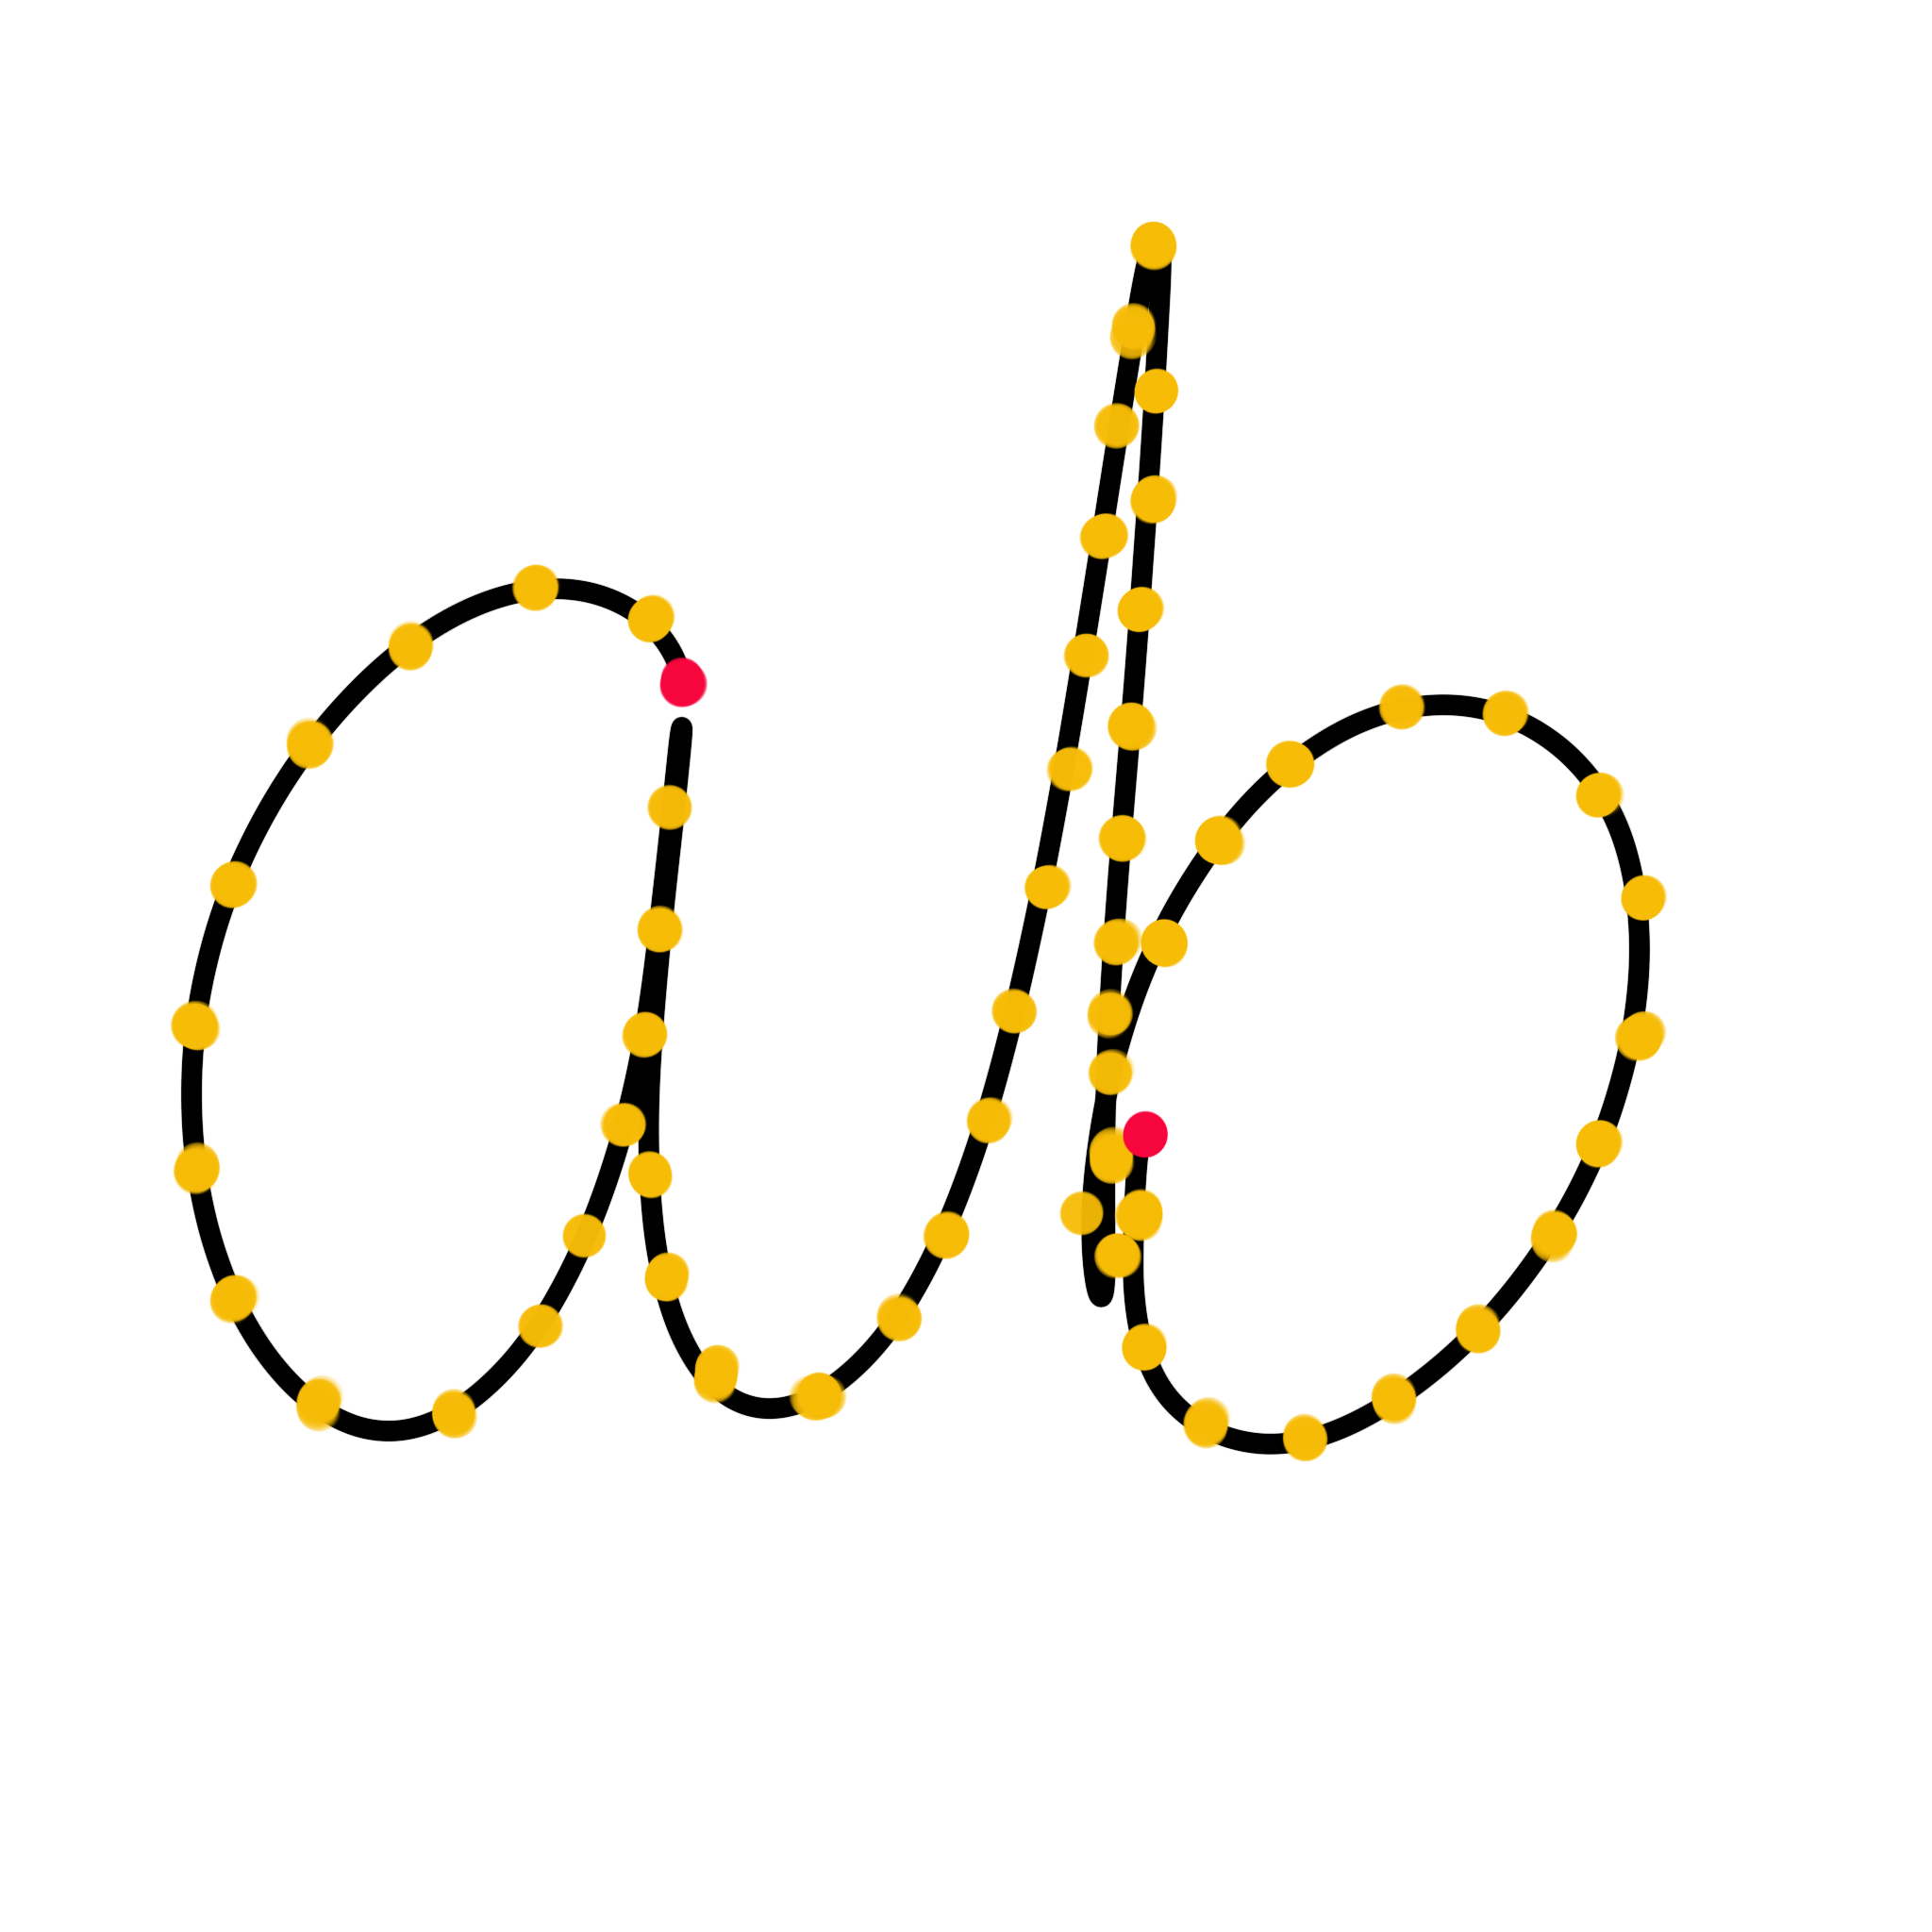
\includegraphics[width=\textwidth]{ab_plots.png}
    \caption{plots}
    \label{abdots}
  \end{minipage}
\end{figure}

%https://mattatlincoln.github.io/teaching/numerical_methods/lecture_5/#/1 

\subsection{Lagrange }
%not yet complete, references to be found 

The first method we look at is Lagrange interpolation to set the foundations for using interpolation in image recognition. Lagrange interpolation allows us to represent a collection of points as a polynomial using the following: 
\begin{equation} \label{lagrangeeqn}
P(x) = \displaystyle\sum_{i=1}^n P_i (x) y_i
\end{equation} % https://brilliant.org/wiki/lagrange-interpolation/

where $P_i(x) = \frac{f(x)}{(x-x_i)f'(x_i)}$ and $f(x) = (x - x_1)(x - x_2) ... (x-x_n)$ \\ 

We begin with an example. 

%Polynomial $P(x)$ of degree less than $ \le $ $(n - 1)$ passes through the points $(x_n, y_n)$ where n starts at 1, $y = f(x_n)$\\ 

%$P_j(x) = y_j \Pi _k = 1  $

%\Pi_{\substack{k = 1\\k \neq j}} \frac{x-x_k}{x_j - x_k} %sort this out - looks horrible 

\begin{figure}[!h]
  \centering
 \begin{minipage}[b]{0.4\textwidth}
 
    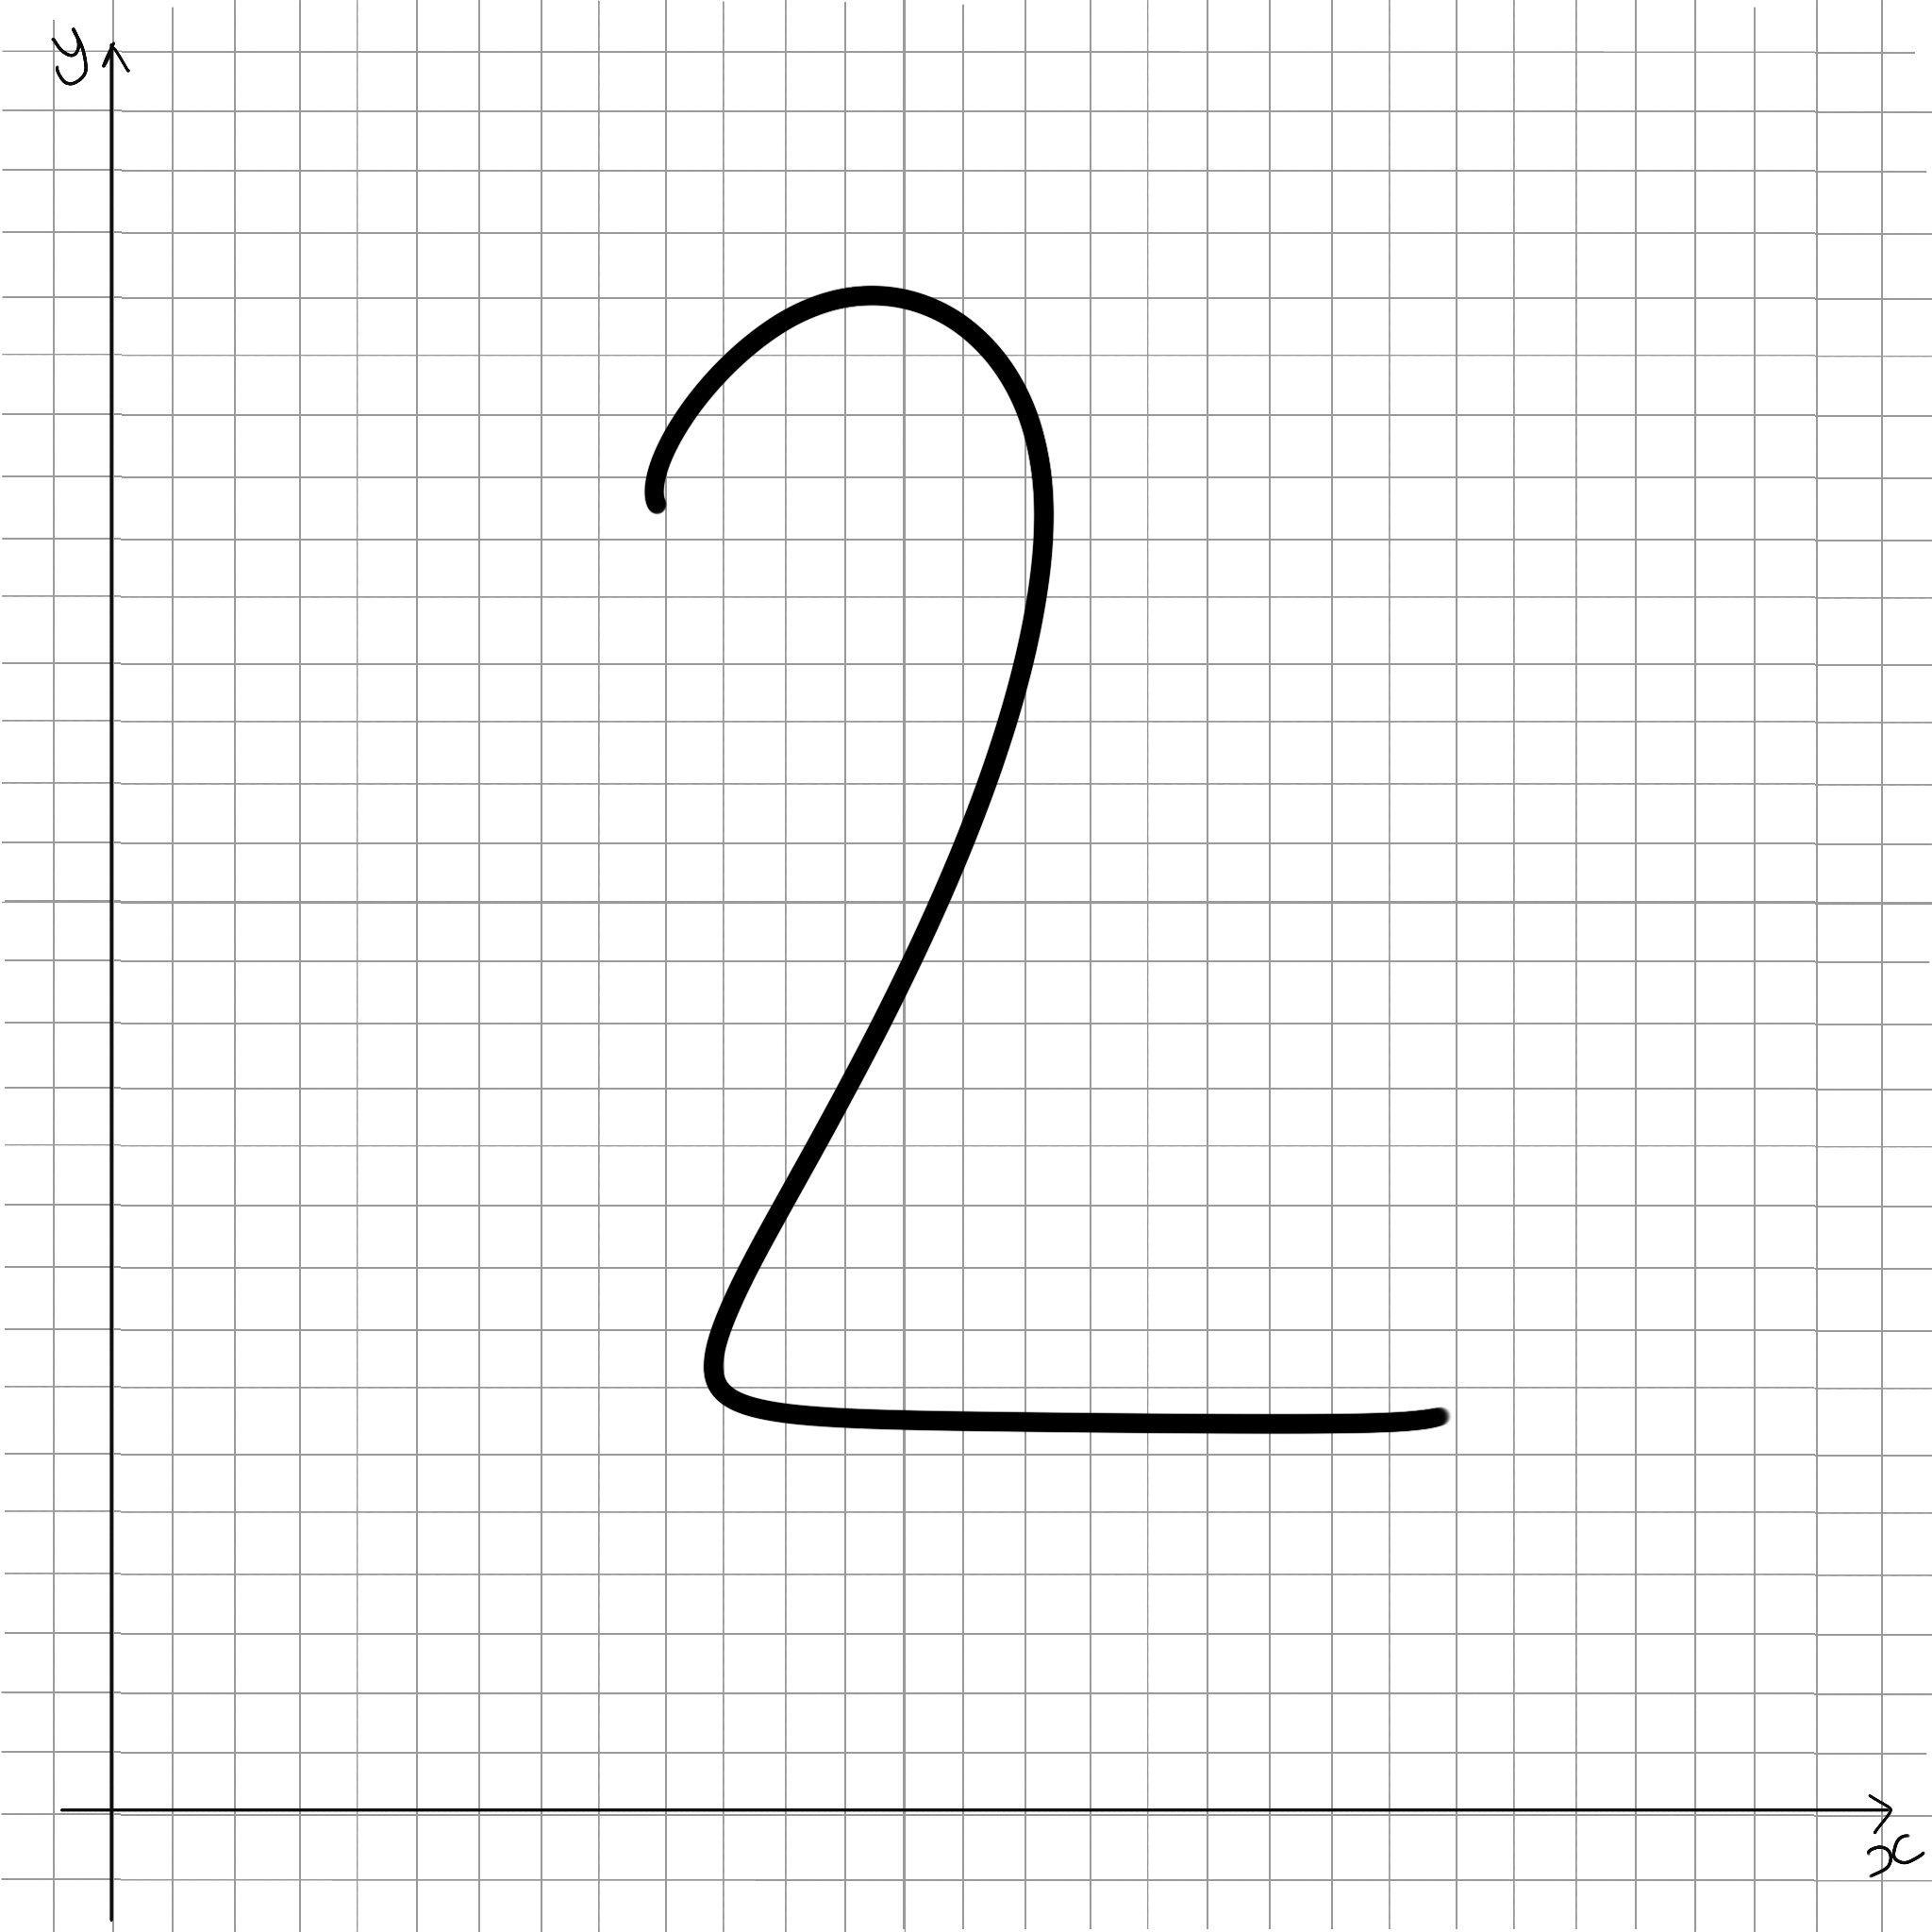
\includegraphics[width=\textwidth]{2graph.png}
      \caption{ }
      \label{2graph}

 \end{minipage}
  \hfill
\begin{minipage}[b]{0.4\textwidth}
    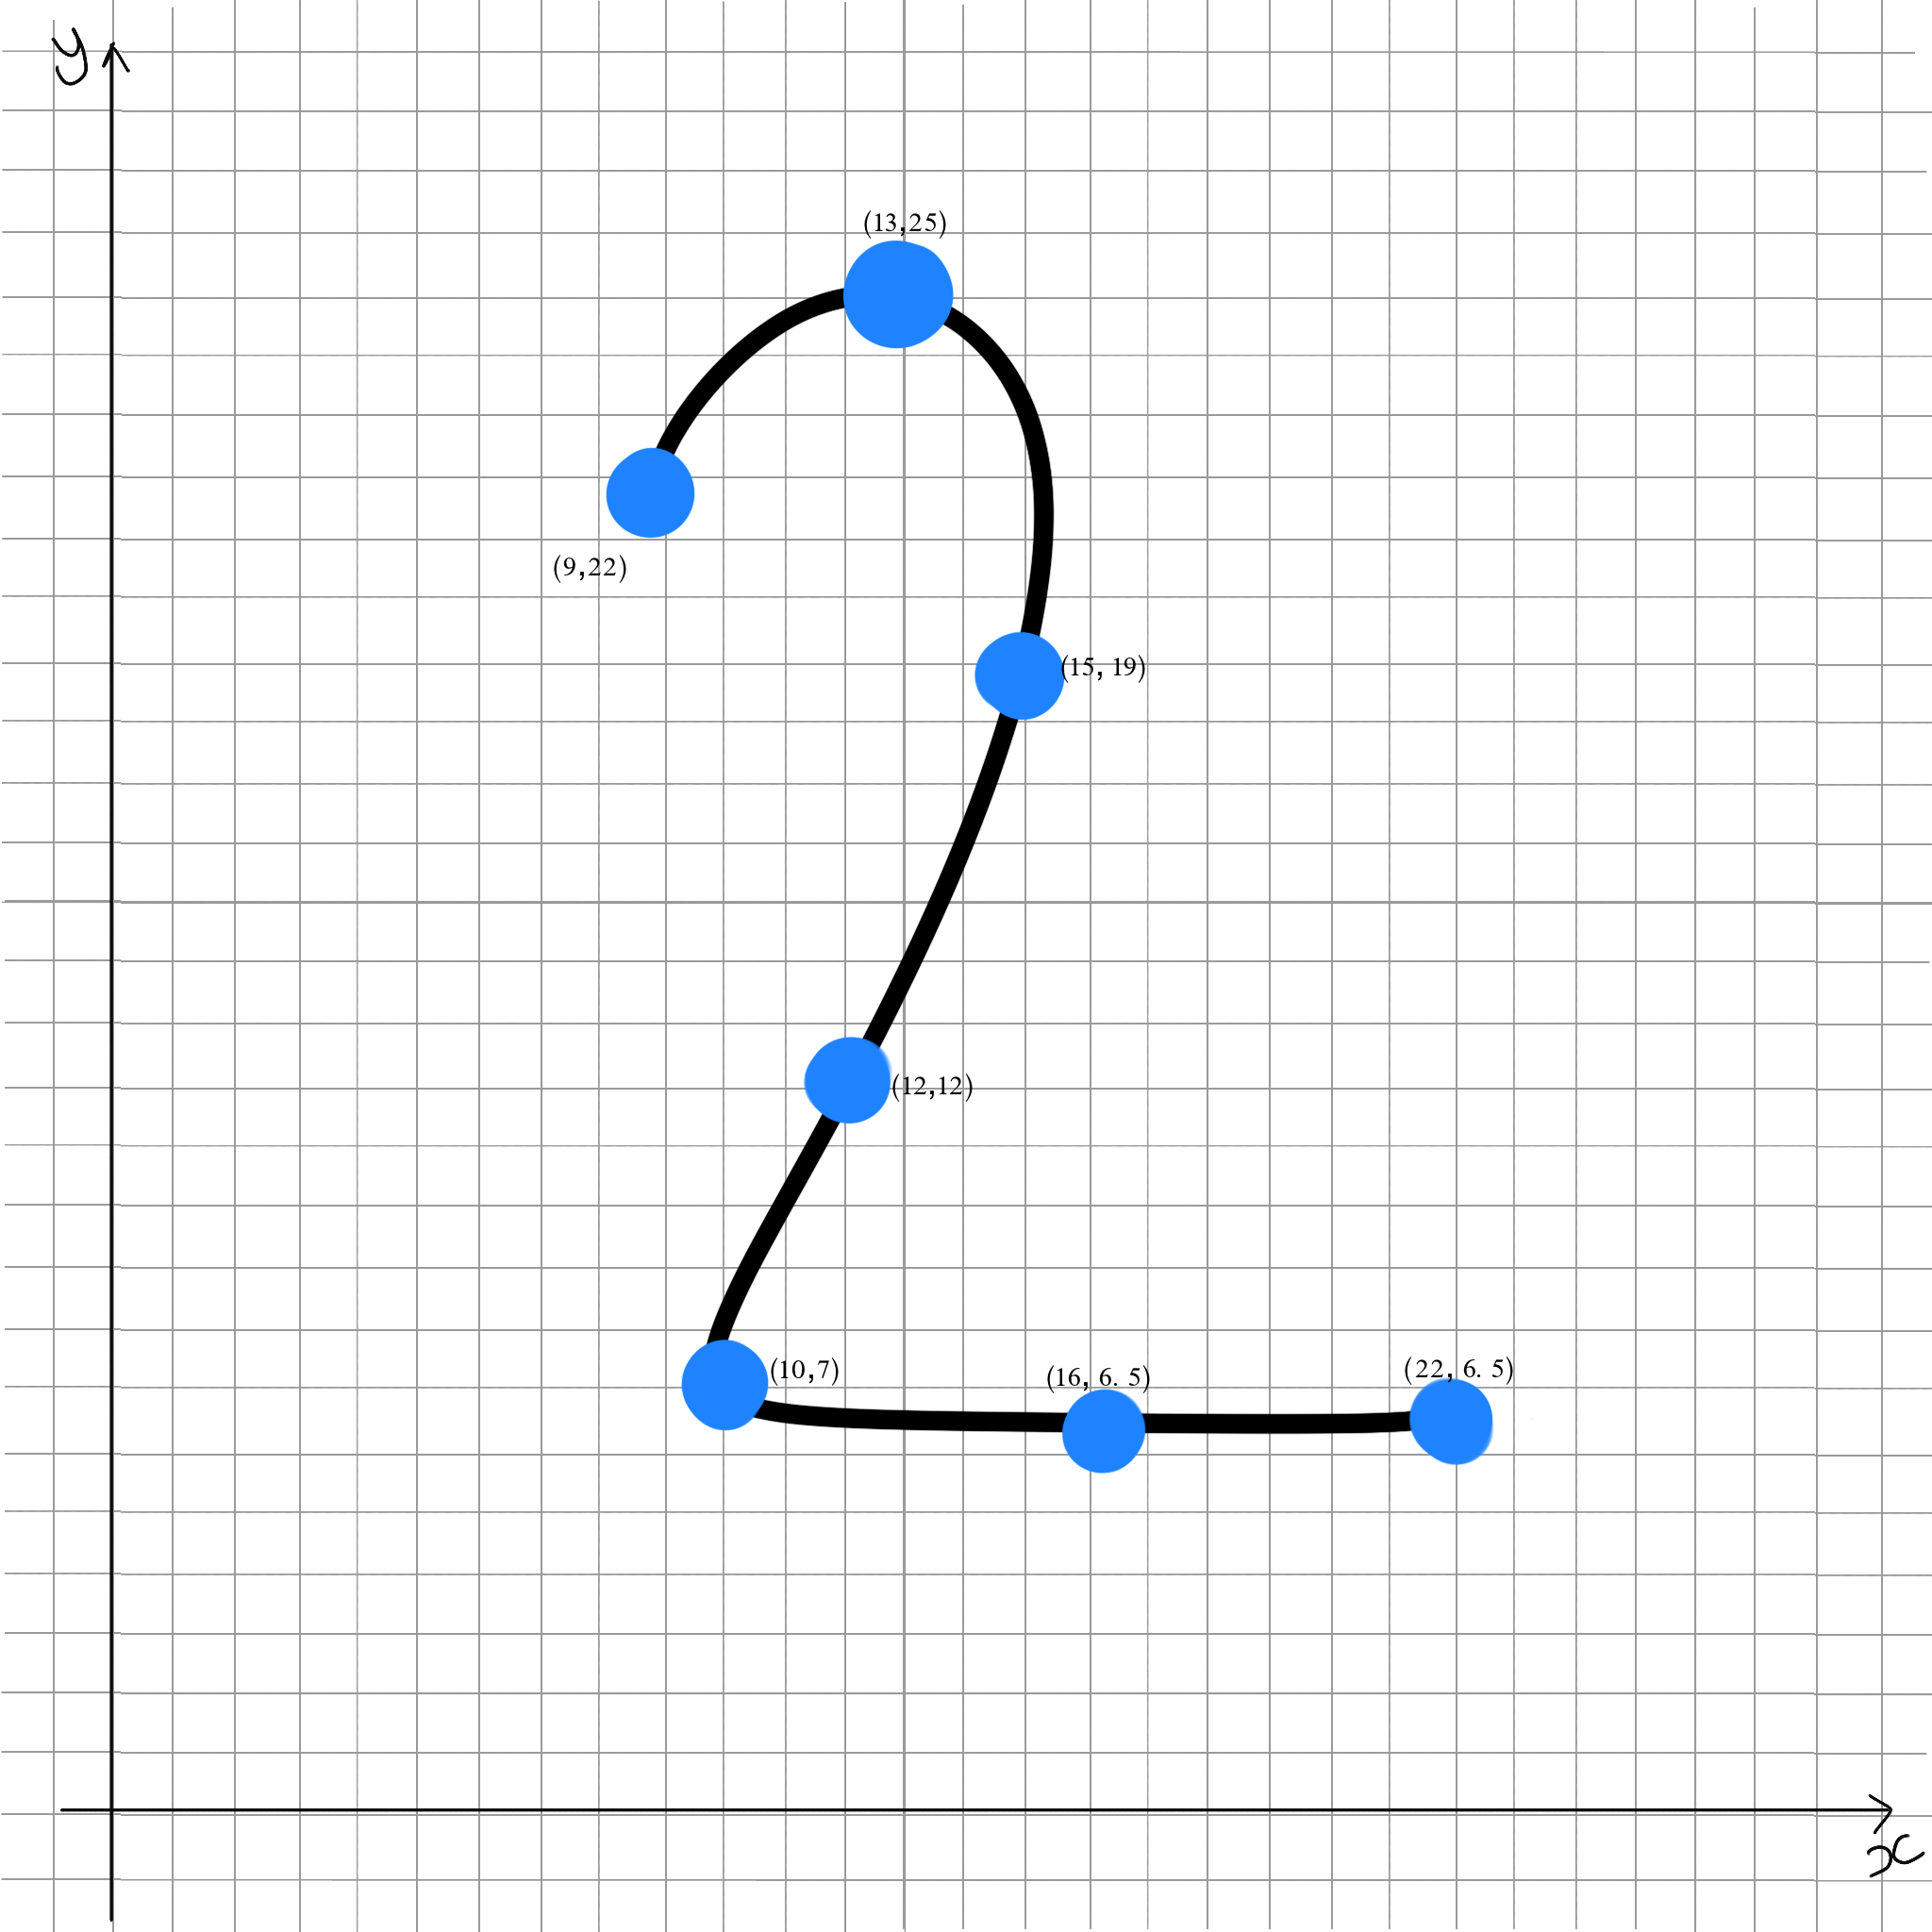
\includegraphics[width=\textwidth]{2graphwplots.png}
      \caption{ }
      \label{2graphwplots}
    \end{minipage}
\end{figure}

\begin{example} \label{lagrangeeg}
Consider figure \ref{2graph}. We begin by taking 7 random points, as displayed in figure \ref{2graphwplots}: \\ 

(9,22), (13, 25), (15, 19), (12, 12), (10, 7), (16, 6.5), (22, 6.5).  \\

Using equation \ref{lagrangeeqn}: 
$P(x) = -0.00885565x^6 + 0.747309x^5 - 25.6916x^4 + 460.525x^3 - 4538.94 x^2 + 2332.1x - 48805.2$ 

(see section \ref{lagrangeegcalc} for full calculation). 
\end{example}

Considering the polynomial $P(x)$ from \ref{lagrangeeg}, we see that the graph does not exist within the area the plots are taken from (roughly the square connecting the points $(9, 6), (9, 25), $ $(23, 25), (23, 6)$). This is likely down to our small selection of points. However, including more points may become problematic, as the increased points will increase the degree of our polynomial $P(x)$; increasing the difficulty and time for calculation. There is the possibility of using a programming language, such as Python \cite{pythonLag} to overcome this. However, what is it we are looking for? We may be able to replicate the digits with polynomials to look similar - but that doesn't get us any closer to recognising the image other than with the human eye. Rather, we move onto another method of interpolation, Chebyshev polynomials. 


\subsection{Chebyshev \label{chebyshev}}
Chebyshev polynomials are orthogonal polynomials used in many function approximation situations.  I have found numerous texts\cite{brilliantCheby}, \cite{oxfordCheby} supporting the use of Chebyshev polynomials, especially for more complex functions. However, the main text I focus on is that by Char and Watt \cite{Chebyshev}. \\ 

We will first explore what Chebyshev polynomials are, and some foundations necessary to use them in image recognition. A chebyshev polynomial of degree $n$ is given by the formula $T_n(x) = \cos(n \cos^{-1} x) $ ,\cite{NumRec}. We may express this as: 
\begin{equation} \label{chebyshevEqn}
T_n(\cos \theta) = \cos n \theta
\end{equation}
such that 
$T_0(x) = 1$ 
$ T_1(x) = x$
$ T_2(x) = 2x^2 - 1 $
$ T_3(x) = 4x^3 -3x$
$ ... $ 
See \ref{chebyshevproofs} for a step-by-step to the above. \\ 

Using equation \ref{chebyshevEqn}, we may obtain \textit{(see appendices, section \ref{chebyshevproofs}) }the following recurrence relation: 
\begin{equation} \label{chebyshevEqn_n+1}
T_{n+1} (x) = 2x T_n(x) - T_{n-1}(x)
\end{equation}

\subsubsection{Using Chebyshev Polynomials to approximate functions }
\label{ChebyshevInterpolation} 

A typical polynomial is of the form $f(x) = ax^n + bx^{n-1} + ... + yx + h$ where $a, b, y, h, n \in \mathbb{R}$. In essence, linear combinations of $1, x, x^2, x^3, ...$. To use Chebyshev polynomials, we consider our functions as linear combinations of $T_n(x)$. \\

For any function f(x'), we express it as \cite{Chebyshev}: 
\begin{equation} \label{sigmaCheby}
f(x') = \Sigma c_k T_k(u) 
\end{equation}
where $u = \frac{2x' - a - b }{b - a}, x' \in [a,b]$. \\ 

We use the transformation  $u = \frac{2x' - a - b }{b - a}$, as it maps $x' \in [a,b]$ to $u \in [-1,1]$, as required by the definition of Chebyshev polynomials, equation \ref{chebyshevEqn}. Equation \ref{sigmaCheby} allows us to solve for the coefficients, $c_k$; this can be done using Chebyshev nodes:
\begin{equation} \label{nodes}
x_i = cos( \frac{2i - 1}{2n} \pi ), i = 1, ..., n
\end{equation} where $x_i$ is the root of $T_n(x)$. 
%https://www.embeddedrelated.com/showarticle/152.php#:~:text=To%20approximate%20a%20function%20by,2%20for%20all%20other%20k. 

\begin{example} \label{chebyshevPolys}
Let $f(x) = 2x^4 + 3x^3 - 2x^2 + x,    x\in [-2, 1]$. We will approximate f(x) using a linear combination of Chebyshev polynomials for $N = 0,1,2,3,4$ 

We use the translation $u = \frac{2x - a - b }{b - a} = \frac{2x -1 }{3}$ . \\ 

Using equation \ref{nodes}, we obtain the Chebyshev nodes (to 3.s.f): 
\begin{itemize}
\item $u_1 = cos( \frac{1}{10} \pi )  = 0.951$, 
\item $u_2 = cos( \frac{3}{10} \pi )  = 0.588$, 
\item $u_3 = cos( \frac{5}{10} \pi )  = 0$, 
\item $u_4= cos( \frac{7}{10} \pi )  = -0.588$,
\item $u_5 = cos( \frac{9}{10} \pi )  = -0.951$ \\
\end{itemize}
\newline
Next, we use $u = \frac{2x -1 }{3}$ to obtain the respective $x$ values, and then input this in to $f(x)$ to obtain the corresponding values of y = f(x). Using values of f(x), and calculating our values of $c_n$ from equation \ref{sigmaCheby}, we may approximate $f(x)$ as follows: \\
$f(x) = 10.5 T_0(u) + 21.1T_1(u) + 11.5 t_2(u) + 5.91 T_3(u) + 1.07 T_4 (u)$, or 
$f(x) = 8.56x^4 + 23.64x^3 + 14.44x^2 + 3.37x + 0.07$ \\ 
\newline 
Full working in section \ref{chebyshevPolysFULL} in the appendices. 
\end{example}


\subsubsection{Image Recognition using Chebyshev Polynomials}
Starting with our handwritten digit, we take continuous plots as the writer draws, similar to \ref{2graphwplots}, but with more points. However, we record the trace now as a sequence of $(x_i, y_i, t_i)$, where $t_0 = 0, t_1 = 1$. I.e. the pen hits the interface at  $t = 0$, and finishes/lifts off at $t = 1$. \\ 

We use linear interpolation on $x$ and $y$ separately from our traces, $(x_i, y_i, t_i)$, to obtain $X(t) = x_i + \frac{x_{i+1} - x_i}{t_{i+1} -t_i}$  and $Y(t) = y_i + \frac{y_{i+1} - y_i}{t_{i+1} -t_i}, t_i \leq t < t_{i+1}$ . Using this, we create the Chebyshev Series:
\begin{equation} \label{chebyXYseries}
X(t) = \Sigma _{i=0} ^ {\infty}  \alpha  _i T_i(t), Y(t) = \Sigma _{i=0} ^{\infty} \beta _ i T_i(t) 
\end{equation}

From here, the reader may use the techniques discussed in section \ref{ChebyshevInterpolation}, and example \ref{chebyshevPolys}, to obtain the coefficients $\alpha _i$ and $\beta _ i$ for equation \ref{chebyXYseries}. The series approximations of $X$ and $Y$ may then be compared with others and classified, using techniques not covered in this report. Future work beyond this report should expand upon this. 

\newpage
\section{Creating Data Sets \label{gatheringdataset}}

As discussed in the introduction, section \ref{datasets}, we have used the MNIST database \cite{MNIST} for handwritten digits. We will discuss now how to capture such data ourselves, from the grayscale values of $28$ x $28$ pixel images, to coordinates as seen in \ref{graphPlots}. 

\subsection{Grayscale Pixel Values }
To capture data manually, we may use Excel, or another similar worksheet tool. For example, figure \ref{excelgrays} shows an excel spreadsheet restricted to 28 rows and 28 columns, with possible inputs $[0,1]$. We can use this to represent images and their pixel grayscale values by 'drawing' the digit directly into the spreadsheet \ref{excelgrays2proper}, or by putting your image in the background and inputting the corresponding values, as done in figure \ref{excelgrays2proper} using figure \ref{2graph}. This, however, is not practical.  \\

To automate this process, increasing processing time and removing human error, we may use a coding language, such as Python, and import the pixel values. %Say we use Python, we can import the pixel values from an image; see appendices: \ref{pixelValCode} 

\begin{figure}[!h]
  \centering
  \begin{minipage}[b]{0.4\textwidth}
    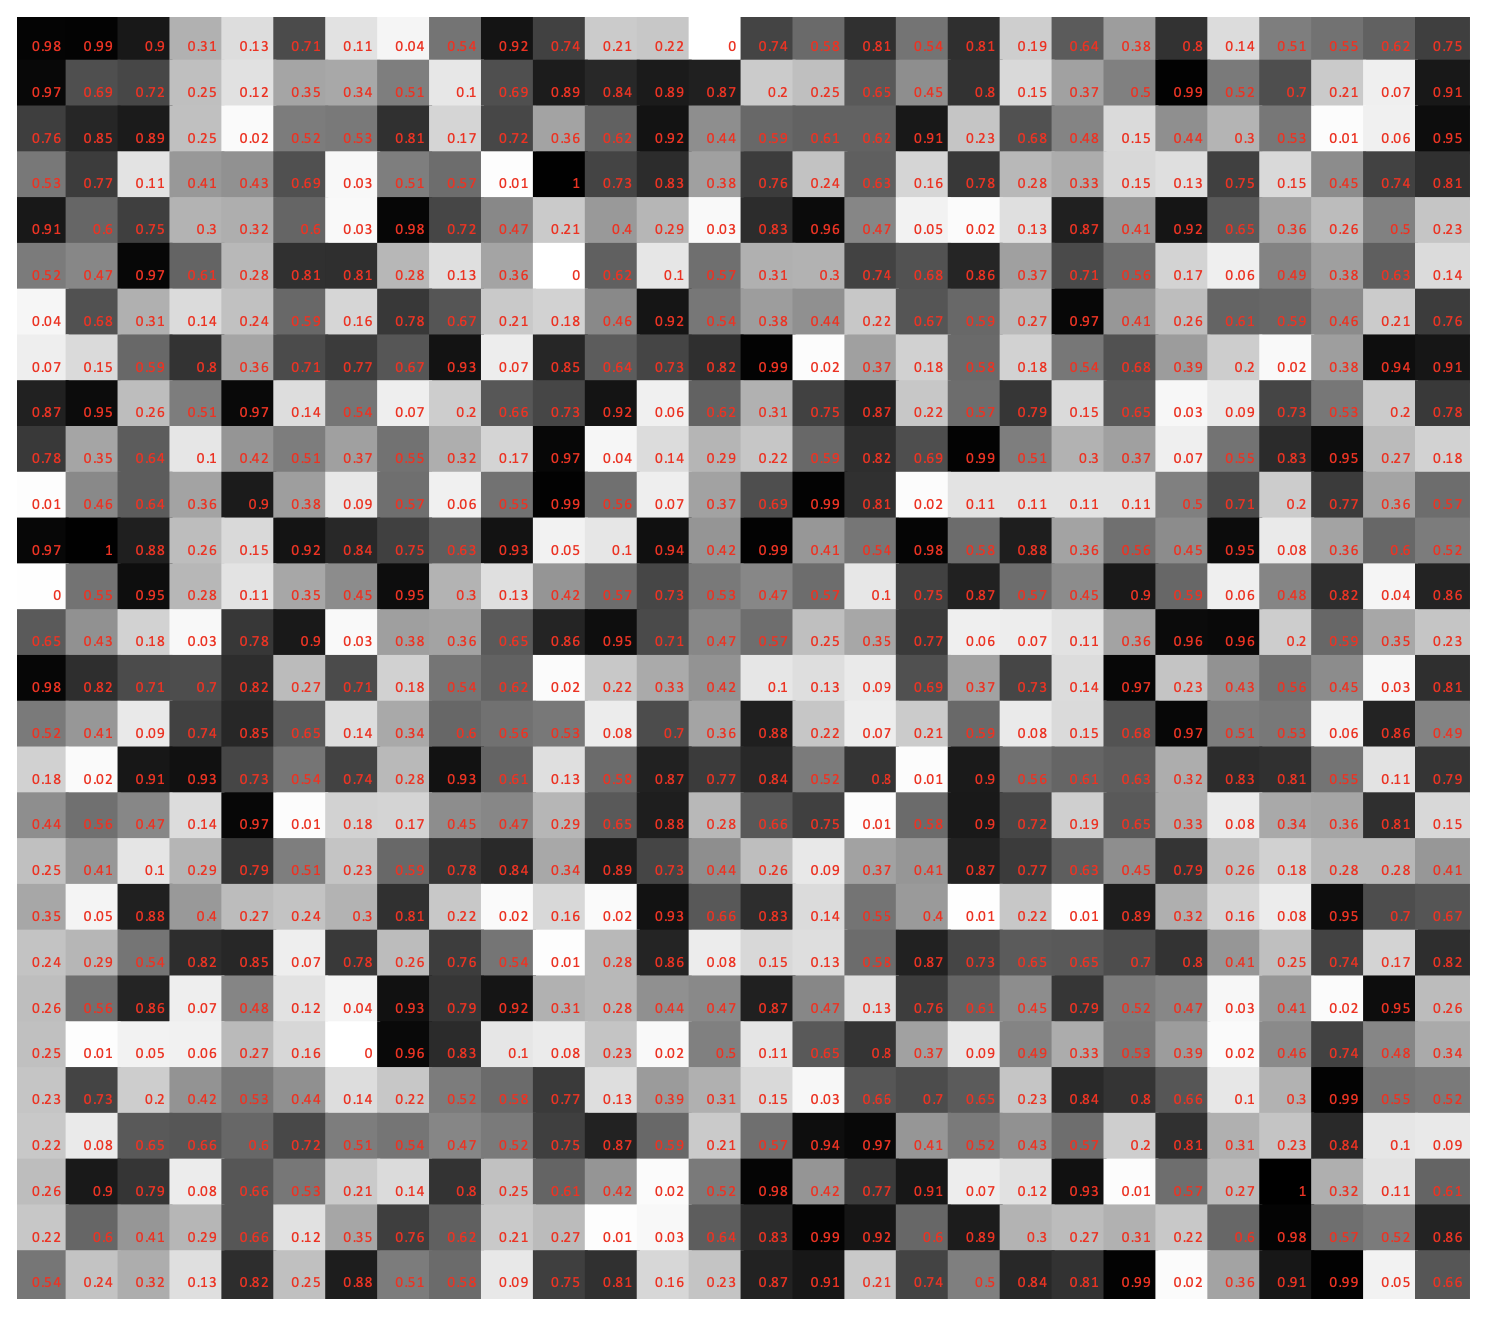
\includegraphics[width=\textwidth]{randomexcel.png}
    \caption{Random grayscale image in excel}
	\label{excelgrays}
  \end{minipage}
  \hfill
 % \begin{minipage}[b]{0.4\textwidth}
    %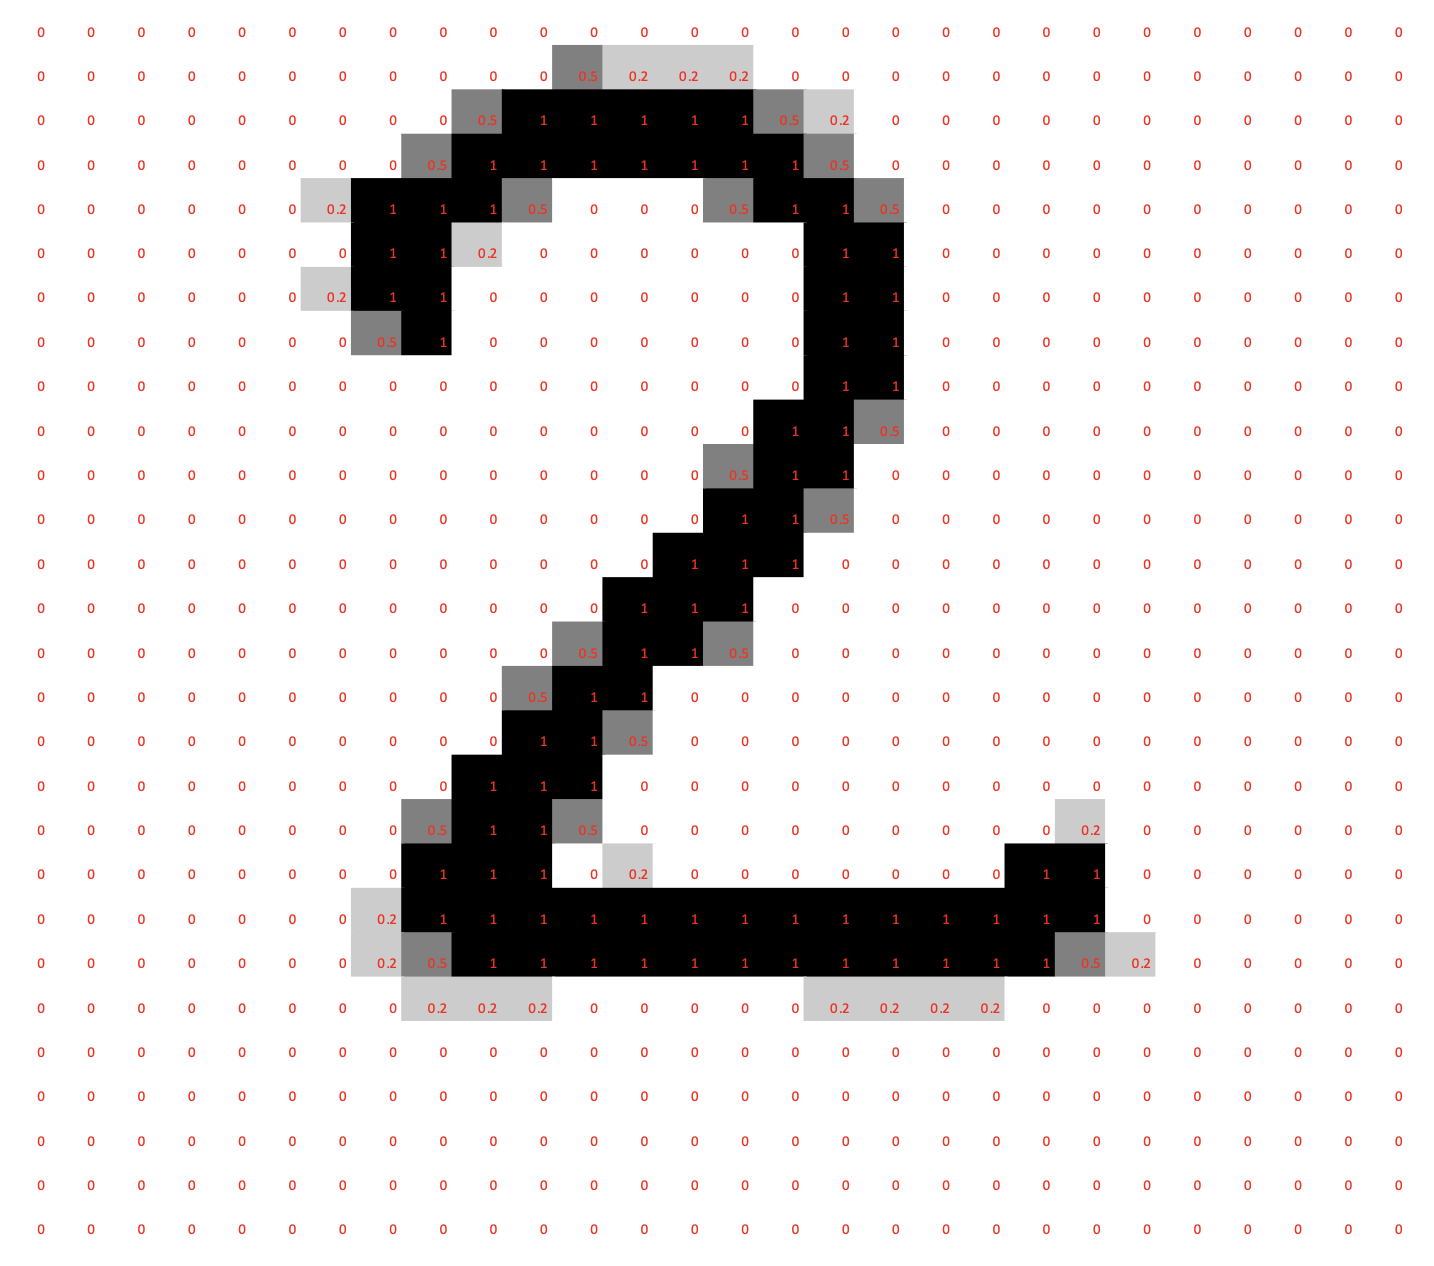
\includegraphics[width=\textwidth]{2excel.png}
   % \caption{Digit 2 grayscale in excel}
   % \label{excelgrays2}
  %\end{minipage}
  %\hfill 
    \begin{minipage}[b]{0.4\textwidth}
    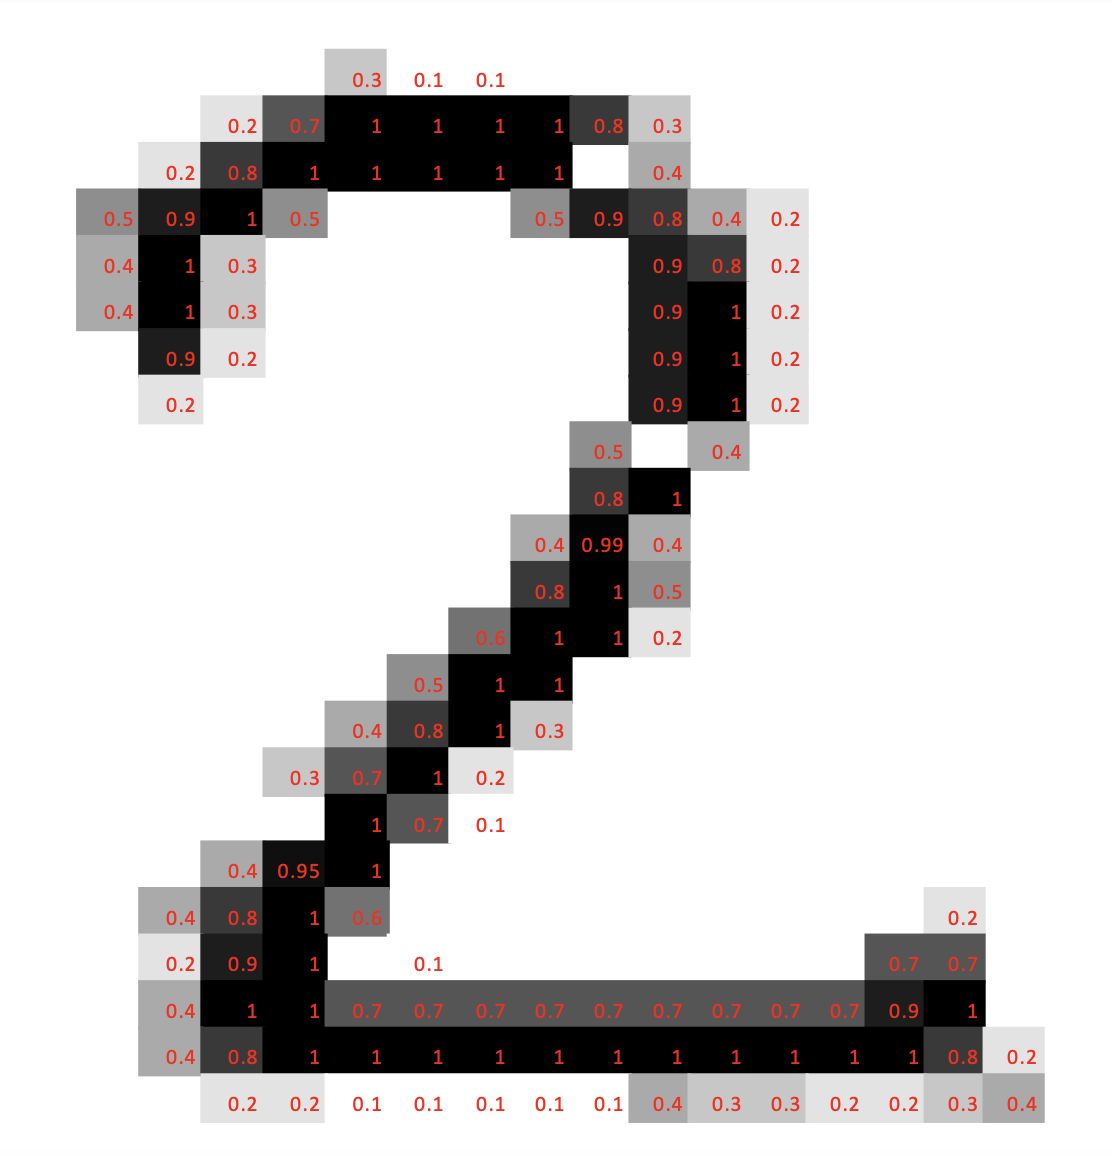
\includegraphics[width=\textwidth]{proper2excel.png}
    \caption{Digit 2 in Excel}
    \label{excelgrays2proper}
  \end{minipage}
 
\end{figure}


\subsection{Graph Plots }
\label{graphPlots} 

For graph plotting, there are tools \cite{WolframCoords} to manually record coordinates from images. Alternatively, we can overlay an xy axis over images and determine their coordinates. When requiring points in the form $(x_i, y_i, t_i)$, it is also necessary to record the time of a trace, and then normalise this to be within the range $[0,1]$. There are, however, tools to automate this process. We shall explore a particular example next, section \ref{InkML}. \\ 

\subsubsection{InkML }
\label{InkML}
InkML uses an electronic pen-based interface, such as a tablet, to track pen movements, recording their $(x, y )$ coordinates to create a sequence. An example of an InkML file is below \cite{INKML}. We may then collate this data with several handwriting samples to create our database ready for interpolation. 

\begin{lstlisting} 
<ink xmlns="http://www.w3.org/2003/InkML">
   <trace>
      10 0, 9 14, 8 28, 7 42, 6 56, 6 70, 8 84, 8 98, 8 112, 9 126, 10 140,
      13 154, 14 168, 17 182, 18 188, 23 174, 30 160, 38 147, 49 135,
      58 124, 72 121, 77 135, 80 149, 82 163, 84 177, 87 191, 93 205
   </trace>
   <trace>
      130 155, 144 159, 158 160, 170 154, 179 143, 179 129, 166 125,
      152 128, 140 136, 131 149, 126 163, 124 177, 128 190, 137 200,
      150 208, 163 210, 178 208, 192 201, 205 192, 214 180
   </trace>
   <trace>
      227 50, 226 64, 225 78, 227 92, 228 106, 228 120, 229 134,
      230 148, 234 162, 235 176, 238 190, 241 204
   </trace>
   <trace>
      282 45, 281 59, 284 73, 285 87, 287 101, 288 115, 290 129,
      291 143, 294 157, 294 171, 294 185, 296 199, 300 213
   </trace>
   <trace>
      366 130, 359 143, 354 157, 349 171, 352 185, 359 197,
      371 204, 385 205, 398 202, 408 191, 413 177, 413 163,
      405 150, 392 143, 378 141, 365 150
   </trace>
</ink>
\end{lstlisting}

\newpage
\section{Conclusion }
We have seen how we may train and use ANNs to classify digits from a dataset throughout this report. We explored how to structure a practical ANN to cater to our needs in section \ref{structure} and created an optimised network in example \ref{handwritingEG}. Using stochastic gradient descent in section \ref{backPropagation}, we saw how we might use the proposed network to develop a NN from our set of training data. \\ 

In section \ref{types}, we saw the different types of neural networks and how they may be used within image recognition. We saw the use of autoencoders to regenerate digits from our network post-training. Later, in section \ref{Sobel}, we saw how we might use edge detection filters to enhance the outputs of autoencoders. Future studies may focus on the impact of combining the two processes.  \\ 

For interpolation methods in section \ref{interpolation}, I focussed on Chebyshev polynomials. Given more time, I would have determined a process to use these from the initial data sets to the final classification result. I would recommend future studies include more profound research on this, as well as exploring other methods of interpolation, such as splines which were mentioned by Marsland \cite{Marsland}.  \\ 

Additionally, there are factors within this project that could affect the classification process that we have accepted following the recommendation from literature. For example, we use the sigmoid function, section \ref{sigmoid}, for our ANNs. However, we did not practise using alternatives, such as ReLU, to assess the impact mathematically. Future studies may compare methods such as this and their suitability. Additionally, variables such as $\eta$ and the number of nodes should be scrutinised similarly.  \\ 

From the report's contents, we have a robust process that is statistically proven to classify handwritten digits: neural networks. In hindsight, I should have spent more time on interpolation. This appears to be an emerging method with more room to develop by changing the interpolation method or adapting the parameters used.  \\ 

This project aimed to understand how mathematics may be used to process and classify images. We have established two methods to classify images: interpolation and neural networks and developed a thorough understanding of these. To better understand the two methods' performance compared, further studies may address the process of image recognition from start to end, using additional tools such as InkML and autoencoders.  \\ 

Overall, I hope you have developed an understanding of the variety of methods available to mathematically categorise handwriting. Thank you for reading. \\ 

\newpage
\section{Acknowledgements}
I want to take this opportunity to thank my partner, Sam Robertson, for keeping me sane and on track with my studies and for simply everything you do for me. Your enthusiasm when listening to the mathematics of image processing cannot be matched. I can't wait to return the favour and support you throughout your physics degree, and I look forward to seeing your final year report within the school in the years to come. Again, thank you. \\ 

I'd also like to thank my parents, Sharon and Wes, for their support throughout my undergraduate studies. From helping with applications to University in 2017 to supporting me with love and encouragement to return to studies in 2019. \\ 

Finally, thank you to my best friends, Anya and Oscar, for always listening to my maths orientated talks and providing endless emotional support. \\ 

I cannot thank you all enough for the love and support you have given me. 
\newpage
\section{Appendices}
\subsection{Research Plan} \label{researchP}
\begin{center}
    \includepdf[pages=-,pagecommand={},width=\textwidth]{Research_plan.pdf}
\end{center}
\newpage
\subsection{Sobel Filter Poster} \label{SobelPoster}
%CHANGE NAME OF BELOW 


\subsection{Calculations}

\subsubsection{Proving equation \ref{dc/dw} }
\label{provingdc/dw}
$z^L = w^L a^{L-1} + b^L  \Rightarrow \frac{\partial z^L}{\partial w^L} = a^{L-1}$

$a^L = \sigma (z^L)  \Rightarrow \frac{\partial a^L}{\partial z^L} =\sigma ' (z^L)$ 

$C_0 = (a^L - y)^2 \Rightarrow \frac{\partial C_0}{\partial a^L} = 2(a^L - y)$

\subsubsection{Example \ref{lagrangeeg} calculations \label{lagrangeegcalc}}


$P(x) = \frac{(x-13)(x-15)(x-12)(x-10)(x-16)(x-22)}{(9 - 13)( 9 - 15)( 9 - 12)( 9 - 10)( 9 - 16)( 9 - 22)}22 +  $ \\ 
\indent $\frac{(x-9)(x-15)(x-12)(x-10)(x-16)(x-22)}{( 13 - 9)( 13 - 15)( 13 - 12)( 13 - 10)( 13 - 16)( 13 - 22)}25 + $ \\ 
\indent $ \frac{(x-9)(x-13)(x-12)(x-10)(x-16)(x-22)}{( 15 - 9)(15 - 13)( 15 - 12)( 15 - 10)( 15 - 16)( 15 - 22)}19  +$ \\
\indent $\frac{(x-9)(x-13)(x-15)(x-10)(x-16)(x-22)}{( 12 - 9)(12 - 13)( 12 - 15)( 12 - 10)( 12 - 16)( 12 - 22)}12  + $ \\
\indent $\frac{(x-9)(x-13)(x-15)(x-12)(x-16)(x-22)}{( 10 - 9)(10 - 13)( 10 - 15)( 10 - 12)( 10 - 16)( 10 - 22)}7 + $ \\
\indent $\frac{(x-9)(x-13)(x-15)(x-12)(x-10)(x-22)}{( 16 - 9)(16 - 13)( 16 - 15)( 16 - 12)( 16 - 10)( 16 - 22)}6.5 + $ \\
\indent $\frac{(x-9)(x-13)(x-15)(x-12)(x-10)(x-16)}{( 22 - 9)(22 - 13)( 22 - 15)( 22 - 12)( 22 - 10)( 22 - 16)}6.5 $ \\



$P(x) = \frac{(x-9)(x-15)(x-12)(x-10)(x-16)(x-22)}{-648}25 + $\\
\indent $\frac{(x-9)(x-13)(x-12)(x-10)(x-16)(x-22)}{1260}19  + $\\
\indent $\frac{(x-9)(x-13)(x-15)(x-10)(x-16)(x-22)}{720}12  + $ \\
\indent $\frac{(x-9)(x-13)(x-15)(x-12)(x-16)(x-22)}{-2160}7 + $\\
\indent $\frac{(x-9)(x-13)(x-15)(x-12)(x-10)(x-22)}{-3024}6.5 + $ \\
\indent $\frac{(x-9)(x-13)(x-15)(x-12)(x-10)(x-16)}{589680}6.5 $ \\


$P(x) = \frac{(x-9)(x-13)(x-15)(x-12)(x-10)(x-16)(x-22)}{6552(x-9)}22 + $ \\
\indent $\frac{(x-9)(x-13)(x-15)(x-12)(x-10)(x-16)(x-22)}{-648(x-13)}25 + $ \\
\indent $\frac{(x-9)(x-13)(x-15)(x-12)(x-10)(x-16)(x-22)}{1260(x-15)}19  +$ \\
\indent $\frac{(x-9)(x-13)(x-15)(x-12)(x-10)(x-16)(x-22)}{720(x-12)}12  + $ \\
\indent $\frac{(x-9)(x-13)(x-15)(x-12)(x-10)(x-16)(x-22)}{-2160(x-10)}7 + $ \\
\indent $\frac{(x-9)(x-13)(x-15)(x-12)(x-10)(x-16)(x-22)}{-3024(x-16)}6.5 + $ \\
\indent $\frac{(x-9)(x-13)(x-15)(x-12)(x-10)(x-16)(x-22)}{589680(x-22)}6.5 $ \\

$P(x) = (x-9)(x-13)(x-15)(x-15)(x-12)(x-10)(x-16)(x-22) (\frac{22}{6552(x-9)} + $ \\
\indent \indent $ \frac{25}{-648(x-13)} + \frac{19}{1260(x-15)}  + \frac{(12}{720(x-12)}  + \frac{7}{-2160(x-10)} + \frac{6.5}{-3024(x-16)} + \frac{6.5}{589680(x-22)} )$ \\


$P(x) = -0.00885565x^6 + 0.747309x^5 - 25.6916x^4 + 460.525x^3 - 4538.94 x^2 + 2332.1x - 48805.2$ 

\subsubsection{Deducing the Chebyshev polynomial, equation \ref{chebyshevEqn}, section \ref{chebyshev} \label{chebyshevproofs}}

$T_0 (\cos\theta) = \cos(0) = 1 \implies T_0(x) = 1$ 
$T_1(\cos \theta) = \cos(\theta) \implies T_1(x) = x$
$T_2(\cos \theta) = \cos(2\theta) = 2\cos^2 ( \theta) - 1 \implies T_2(x) = 2x^2 - 1 $
$T_3(\cos \theta) = \cos(3\theta) = 4\cos^3(\theta) -3\cos(\theta) \implies T_3(x) = 4x^3 -3x$ 

\subsubsection{Deducing the Chebyshev Recurrence Relation, equation \ref{chebyshevEqn_n+1}, section \ref{chebyshev}} \label{chebyshevproofs}

$T_{n+1}(\cos \theta) = \cos((n +1)\theta)$ 
$\cos((n+1)\theta ) = \cos n\theta \cos\theta - \sin n \theta \sin \theta$ 
$\implies \cos(n+1) \theta + \cos (n-1) \theta = 2\cos \theta \cos n \theta$
$\implies T_{n+1} (x) = 2x T_n(x) - T_{n-1}(x)$
 
\subsubsection{Full workings of equation \ref{chebyshevPolys}}
\begin{example} \label{chebyshevPolysFULL}
$f(x) = 2x^4 + 3x^3 - 2x^2 + x,    x\in [-2, 1]$ 
Using the translation $u = \frac{2x - a - b }{b - a} = \frac{2x -1 }{3}$ 


We then have the following Chebyshev nodes (to 3.s.f): 
$u_1 = cos( \frac{1}{10} \pi )  = 0.951$, 
$u_2 = cos( \frac{3}{10} \pi )  = 0.588$, 
$u_3 = cos( \frac{5}{10} \pi )  = 0$, 
$u_4= cos( \frac{7}{10} \pi )  = -0.588$,
$u_5 = cos( \frac{9}{10} \pi )  = -0.951$,

Using the relation between $u$ and $x$, we may obtain the relevant $x$ values, and then input this in to $f(x)$ to obtain the corresponding values of y = f(x) : 
$y_1 = 43.5, y_2 = 12.8, y_3 = 0.500, y_4 = -0.797, y_5 = -5.56$ 

We then use this to calculate our values of $c_n$ from equation \ref{sigmaCheby}: 
$c_0 = $ average $T_0 y = 10.5$ 
$c_1 = 2 *$ average $T_1y = 2 *$ average $u * y = 21.1$
$c_2 = 2 * $ average $T_2 y = 2 * $ average $(2u^2 - 1) * y = 11.5$ 
$c_3 = 2* $ average $T_3 y = 2* $ average $(4u^3 - 3u) * y = 5.91$ 
$c_4 = 2*$ average $T_4 y = 2 * $ average $(8u^4 - 8u^2 +1) * y = 1.07$ 

Using these values, we may approximate $f(x)$ as follows: $f(x) = 10.5 T_0(u) + 21.1T_1(u) + 11.5 t_2(u) + 5.91 T_3(u) + 1.07 T_4 (u)$, or 
$f(x) = 8.56x^4 + 23.64x^3 + 14.44x^2 + 3.37x + 0.07$
\end{example}
\newpage
\subsection{Code}

\subsubsection{Perceptron Network Code \label{simpleNN}}
\begin{lstlisting}
//Code for simple 'AND' 

#include <stdlib.h>  //for our random numbers
#include <math.h>  //for exp 
#include <iostream>
using namespace std;

//a function for the sigmoid function 
double sigmoid_function(double x) { 
	return 1 / (1 + exp(-1 * x));
}

int main()
{
	
	//cout << w[0] << endl; //w[0] corresponds to A, w[1] corresponds to B, w[2] is for the bias 
	//cout << w[1] << endl;
	//cout << w[2] << endl;

	//defining all variables here to make code clearer
	int expected_output;
	//weights for a&b, and the bias
	double w_a = rand() % 10;
	double w_b = rand() % 10;
	double bias = rand() % 10; 

	//a_L = activation
	double z_L, a_L; 
	double delta_w_a, delta_w_b, delta_b; //dC/dw_a, dC/dw_B, dC/db
	

	for (int i = 0; i < 50000; i++) {

		int A = rand() % 2; //Assign 0, or 1, to A&B
		int B = rand() % 2;

		if (A == 0 && B == 0) {
			expected_output = 0;
		}
		else {
			expected_output = 1;
		}

		cout << "A = " << A << endl;
		cout << "B = " << B << endl;

		cout << "w_a = " << w_a << endl;
		cout << "w_b = " << w_b << endl;
		cout << "b = " << bias << endl;

		z_L = w_a * A + w_b * B + bias; 
		a_L = sigmoid_function(z_L); 
		cout << "Expected output: " << expected_output << endl; 
		cout << "----VS----" << endl;
		cout << "Network output: " << a_L << endl;

		//changes to be made 	
		delta_w_a = 2 * A * a_L * (1 - a_L) * (a_L - expected_output); 
		delta_w_b = 2 * B * a_L * (1 - a_L) * (a_L - expected_output);
		delta_b = 2 * a_L * (1 - a_L) * (a_L - expected_output);

		w_a -= delta_w_a;
		w_b -= delta_w_b; 
		bias -= delta_b; 

		
	}
}

\end{lstlisting}

\newpage
\subsubsection{Multilayer Network Code} \label{pixelValCode}

\begin{lstlisting}
#include <iostream>
#include <algorithm> // for transform
#include <functional> // for plus
#include <cmath> 
#include <math.h>
#include <Dense>

using namespace std;
using namespace Eigen;

//sigmoid function 
double sig_fntion(double x) {
    return 1 / (1 + exp(-1 * x));
}

int main()
{
    //describing the NN 
    int no_of_layers = 3; //including input, output, and hidden
    int neurons_input = 4; //number of input neurons, labelled A, B, C, D 
    int neurons_output = 2; //outputs labelled w and b respectively 
    int neurons_h1 = 3; //number in hidden layer, labelled 0 - 2
    int a = neurons_h1 + neurons_output; //the amount of activations from the activation function, input neuron values are not activations here 

    double A, B, C, D; //our inputs 

    int N_w, N_b;
    N_w = neurons_input * neurons_h1 + neurons_h1 * neurons_output; //number of weights
    N_b = neurons_h1 + neurons_output;  //number of biases


    VectorXd w(N_w), b(N_b); //w_0A^L-1, w_0B^L-1, w_0C^L-1, w_0D^L-1, w_1A^L-1, etc. 
     //vector displaying ALL weights 
    for (int i = 0; i < N_w; i++) {
        w(i) = rand() % 10;
    }
    //weights = (w_0A, w_0B, w_0C, w_0D, w_1A, w_1B, w_1C, w_1D, w_2A, w_2B, w_2C, w_2D, w_w0, w_w1, w_w2, w_b0, w_b1, w_b2)

    //vector displaying ALL biases 
    for (int k = 0; k < N_b; k++) {
        b(k) = rand() % 10;
    }

    int out = 2; //no of output neurons
    VectorXd e_out(out); //our expected outputs 
    // e = ['white' 'black'] - 2 neurons, one depicts white, the other depicts black 

    cout << "Beginning program. Intial values of weights: " << endl;
    cout << w << endl;
    cout << "Initial biases: " << endl;
    cout << b << endl;



    for (int i = 0; i < 100000; i++) {

        //our input neurons are A B C D
        A = rand() % 2;
        B = rand() % 2;
        C = rand() % 2;
        D = rand() % 2;

        double average_grayscale_value; //the inputs are grayscale values
        average_grayscale_value = (A + B + C + D) / 4;


        //declare what the outputs should be 
        if (average_grayscale_value > 0.5) {
            e_out << 0, 1; //image mostly black  
        }
        else {
            e_out << 1, 0; //image mostly white 
        }


        //define the activations
        VectorXd activations(a);
        VectorXd z(a); //to work out activations
        for (int q = 0; q < a; q++) {
            activations(q) = 0;
            z(q) = 0;
        }

        //hidden layer:
        for (int m = 0; m < neurons_h1; m++) {
            z(m) = w(4 * m) * A + w(4 * m + 1) * B + w(4 * m + 2) * C + w(4 * m + 3) * D;
        }
        //OUTPUT LAYER
        z(3) = w(12) * z(0) + w(13) * z(1) + w(14) * z(2);
        z(4) = w(15) * z(0) + w(16) * z(1) + w(17) * z(2);


        //therefore all activations:
        for (int t = 0; t < a; t++) {
            activations(t) = sig_fntion(z(t));
        }



        //GRADIENT DESCENT
        VectorXd deltaC_w(N_w), deltaC_b(N_b); //delta cost for C wrt w's, and then b's
         //assign zeros to the above vectors to allow for values to be added
        for (int l = 0; l < N_w; l++) {
            deltaC_w(l) = 0;
        }
        for (int f = 0; f < N_b; f++) {
            deltaC_b(f) = 0;
        }

        //FOR THE OUTPUT LAYER
        // i = all weights - (number of activations)

            //for the 'white' output neuron
        for (int g = N_w - a; g < N_w - a + neurons_h1; g++) {
            deltaC_w(g) = 2 * w(g - 13) * activations(3) * (1 - activations(3)) * (activations(3) - e_out(0));
        }
        //a(3) = activation of the 'white' neuron

        //bias
        deltaC_b(3) = 2 * activations(3) * (1 - activations(3)) * (activations(3) - e_out(0));

        //for the 'black' output neuron
        for (int h = N_w - a + neurons_h1; h < N_w; h++) {
            deltaC_w(h) = 2 * w(h - 16) * activations(4) * (1 - activations(4)) * (activations(4) - e_out(1));
        }

        //bias
        deltaC_b(4) = 2 * activations(4) * (1 - activations(4)) * (activations(4) - e_out(1));

        //HIDDEN LAYER

        VectorXd sum(neurons_h1); //sum = change in C wrt to a^L-1
        sum(0) = w(12) * activations(3) * (1 - activations(3)) * 2 * (activations(3) - e_out(0)) + w(15) * activations(4) * (1 - activations(4)) * 2 * (activations(4) - e_out(1));
        sum(1) = w(13) * activations(3) * (1 - activations(3)) * 2 * (activations(3) - e_out(0)) + w(16) * activations(4) * (1 - activations(4)) * 2 * (activations(4) - e_out(1));
        sum(2) = w(14) * activations(3) * (1 - activations(3)) * 2 * (activations(3) - e_out(0)) + w(17) * activations(4) * (1 - activations(4)) * 2 * (activations(4) - e_out(1));

        //for weights connecting input and hidden 
        for (int i = 0; i < (neurons_h1 * neurons_input); i++) {

            if (i < neurons_input) { //w_0A, w_0B, w_0C, w_0D
                int j = 0;
                if (i % neurons_input == 0) {
                    deltaC_w(i) = A * activations(j) * (1 - activations(j)) * sum(j);
                }
                else if (i % neurons_input == 1) {
                    deltaC_w(i) = B * activations(j) * (1 - activations(j)) * sum(j);
                }
                else if (i % neurons_input == 2) {
                    deltaC_w(i) = C * activations(j) * (1 - activations(j)) * sum(j);
                }
                else if (i % neurons_input == 3) {
                    deltaC_w(i) = D * activations(j) * (1 - activations(j)) * sum(j);
                }
            }

            else if (i < 2 * neurons_input) { //w_1A, w_1B, w_1C, w_1D,
                int j = 1;
                if (i % neurons_input == 0) {
                    deltaC_w(i) = A * activations(j) * (1 - activations(j)) * sum(j);
                }
                else if (i % neurons_input == 1) {
                    deltaC_w(i) = B * activations(j) * (1 - activations(j)) * sum(j);
                }
                else if (i % neurons_input == 2) {
                    deltaC_w(i) = C * activations(j) * (1 - activations(j)) * sum(j);
                }
                else if (i % neurons_input == 3) {
                    deltaC_w(i) = D * activations(j) * (1 - activations(j)) * sum(j);
                }
            }

            else if (i < 3 * neurons_input) { //w_2A, w_2B, w_2C, w_2D,
                int j = 2;
                if (i % neurons_input == 0) {
                    deltaC_w(i) = A * activations(j) * (1 - activations(j)) * sum(j);
                }
                else if (i % neurons_input == 1) {
                    deltaC_w(i) = B * activations(j) * (1 - activations(j)) * sum(j);
                }
                else if (i % neurons_input == 2) {
                    deltaC_w(i) = C * activations(j) * (1 - activations(j)) * sum(j);
                }
                else if (i % neurons_input == 3) {
                    deltaC_w(i) = D * activations(j) * (1 - activations(j)) * sum(j);
                }
            }
        }

        for (int i = 0; i < neurons_h1; i++) {
            deltaC_b(i) = activations(i) * (1 - activations(i) * sum(i));
        }


        //IMPLEMENT CHANGES
        for (int i = 0; i < N_w; i++) {
            w(i) -= deltaC_w(i);
        }

        for (int i = 0; i < N_b; i++) {
            b(i) -= deltaC_b(i);
        }

        double cost_weights = 0;
        double cost_bias = 0;

        for (int i = 0; i < N_w; i++) {
            cost_weights += deltaC_w(i);
        }

        for (int i = 0; i < N_b; i++) {
            cost_bias += deltaC_b(i);
        }

        double cost_total = cost_weights + cost_bias;

        cout << "Cost function = " << cost_bias << endl;
    }

    cout << "Learning complete, values of weights and biases: " << endl;
    cout << "w = " << endl;
    cout << w << endl;

    cout << "b = " << endl;
    cout << b << endl;

    
}
\end{lstlisting}

\newpage
\subsection{Sobel Filter Poster}
\begin{center}
    \includepdf[]{SobelPoster.pdf}
\end{center}


\begin{thebibliography}{}


\bibitem{NN} M.A. Nielsen, \textit{Neural Networks and Deep Learning}, Determination Press, 2015. [Ebook] Available: http://neuralnetworksanddeeplearning.com/chap1.html

\bibitem{SobelFilter} A. Baron, "How Ultra is Sound? Quantifying Images to Refine Diagnosis", Apr. 2021. 

\bibitem{Marsland} S. Marsland, \textit{Machine Learning: An Algorithmic Perspective}, 2nd ed., NY USA, Chapman and Hall, 2014. 

\bibitem{Stathakis} D. Stathakis, (2009). "How many hidden layers and nodes?". Internal Journal of Keynote Sensing, 30:8, 2133-2147, DOI: 10.1090/01431160902549278

\bibitem{Chebyshev} B. W. Char, S. M. Watt, "Representing and Characterizing Handwritten Mathematical Symbols through Succicnt Functional Approximation," in \textit{Ninth International Conference on Document Analysis and Recognition (ICDAR) }, 2007, pp. 1198-1202.

\bibitem{INKML} Y. Chee, K. Franke, M. Fourmentin, S. Madhvanath, J. Magaña, G. Pakos, G. Russell, M. Selvaraj, G. Seni, C. Tremblay, L. Yaeger, “Ink Markup Language (InkML)”, W3C, Sep. 20, 2011. [Online] Available: https://www.w3.org/TR/InkML/

\bibitem{MNIST} L. Den, "The MNIST database of handwritten digit images for machine learning research." \textit{IEEE Signal Processing Magazine}, vol. 29, no. 6, pp 141 - 142, 2012. 

\bibitem{Bain} A. Bain, \textit{ Mind and Body: The Theories of Their Relation.} NY U.S.A.: D. Appleton and Company, 1873. 

\bibitem{James} W. James. \textit{The Principles of Psychology},  NY U.S.A: H. Holt and Company, 1890. 

\bibitem{mcculloch} W. S. McCulloch, W. Pitts, "A Logical Calculus of Ideas Immanent in Nervous Activity", \textit{Bulletin of Mathematical Biophysics}, vol. 5, no. 4, pp.  115–133, Dec. 1943. 

\bibitem{NNforPC} C. M. Bishop, \textit{Neural networks for pattern recognition}, Oxford, UK: Oxford University Press, 1995.

\bibitem{FirstNNbegin}[FirstNNbegin] A. Arnx. (2019, 01.13). First neural network for beginners explained (with code), [Online] Available: https://towardsdatascience.com/first-neural-network-for-beginners-explained-with-code-4cfd37e06eaf

\bibitem{Java} J. Heaton, \textit{Introduction to Neural Networks for Java}, 2nd ed., Chesterfield, MO: Heaton Research Inc, 2008. 
 

\bibitem{BST} H. Samson, "Getting to know Activation Functions in Neural Networks," Towards Data Science, Jun 25, 2020. [Online] Available: https://towardsdatascience.com/getting-to-know-activation-functions-in-neural-networks-125405b67428#:~:text=Binary\%20step\%20function\%20is\%20a,said \\ 
\%20threshold\%20neuron\%20is\%20deactivated.

\bibitem{activationfunc} BP. Baheti, "12 Types of Neural Network Activation Functions: How to Choose," \textit{Deep Learning}, Accessed: May 1, 2022. [Online] Available: https://www.v7labs.com/blog/neural-networks-activation-functions#choose-activation-function

\bibitem{relu} D. Yarotsky, "Error bounds for approximations with deep ReLU networks," \textit{Neural Networks}, vol. 94, pp 103-114, Oct. 2017.  

\bibitem{DeepPy} N. Ketkar, "Stochastic Gradient Descent" in: \textit{Deep Learning with Python}, Berkeley, CA, Apress, 2017.


\bibitem{weightvals} J. Brownlee, " Weight Initialization for Deep Learning Neural Networks," \textit{Machine Learning Mastery, }Feb. 3, 2021. [Online] Available: https://machinelearningmastery.com/weight-initialization-for-deep-learning-neural-networks/#:~:text=Historically\%2C\%20weight\%20initialization \\
\%20follows\%20simple,the\%20range\%20\%5B\%2D1\%2C\%201\%5D

\bibitem{typesNN} Aravindpai, "CNN vs. RNN vs. ANN – Analyzing 3 Types of Neural Networks in Deep Learning", \textit{Analytics Vidhya}, Feb. 17, 2020. [Online} Available: https://www.analyticsvidhya.com/blog/2020/02/cnn-vs-rnn-vs-mlp-analyzing-3-types-of-neural-networks-in-deep-learning/

\bibitem{RNN} W. Yin, K. Kann, M Yu, H. Schutze, \textit{Comparative Study of CNN and RNN for Natural Language Processing}, LMU Munich, Germany, and IBM Research, U.S.A, Feb. 7, 2017. 

\bibitem{CNNHandwriting} A. Poznanski, L. Wolf, "CNN-N-Gram for Handwriting Word Recognition," in 
\textit{IEEE Conference on Computer Vision and Pattern Recognition (CVPR)}, Las Vegas, NV, U.S.A, pp. 2305-2314, 2016. [Online] Available: 
https://openaccess.thecvf.com/content\_cvpr\_2016/html/Poznanski\_CNN-N-Gram\_for\_Handwriting\_CVPR_2016\_paper.html 


\bibitem{GAN} A. Creswell, T. White, V. Dumoulin, K. Arulkumaran, B. Sengupta, A. A. Bharath, "Generative Adversarial Networks: An Overview," \textit{IEEE Signal Processing Magazine}, vol. 35, no. 1, pp 53 - 65, Jan. 2018

\bibitem{autoenc} W. Badr, Auto-Encoder: "What Is It? And What Is It Used For? (Part 1)," \textit{Towards Data Science}, Apr. 22, 2019. [Online] Available: https://towardsdatascience.com/auto-encoder-what-is-it-and-what-is-it-used-for-part-1-3e5c6f017726 

\bibitem{DKL} S. Kullback, R.A. Leibler, "On information and sufficiency," \textit{Annals of Mathematical Statistics}, vol. 22, no. 1, pp 79-86,  22 (1): 79–86, Mar. 1951. 

\bibitem{EdgeDetecImage} T. Yang, Y. H. Qiu, "Improvement and implementation for Canny edge detection algorithm" in \textit{Seventh International Conference on Digital Image Processing (ICDIP)}, Jul. 6, 2015. 

\bibitem{sobel} I. Sobel, \textit{An Isotropic 3x3 Image Gradient Operator}, Presentation at Stanford A.I. Project, 1968. [Online] Available: https://www.researchgate.net/publication/239398674\_An\_Isotropic\_3x3
\_Image\_Gradient\_Operator

\bibitem{edgePDF} D. Ziou, S. Tabbone, "Edge detection techniques: An overview,"\textit{ International Journal of Patttern Recognition and Image Analysis}, vol. 4, pp 537-559, 1998. 

\bibitem{sobelIs} S. Sodha, "An Implementation of Sobel Edge Detection," \textit{Project Rhea}, 2017. [Online] Available: 
https://www.projectrhea.org/rhea/index.php/An\_Implementation\_of \\
\_Sobel\_Edge\_Detection

\bibitem{onlinefilters} Online Edge Detection, \textit{Pine Tools}. [Online], Available: https://pinetools.com/image-edge-detection

\bibitem{pythonLag} Q. Kong, T. Siauw, A. Bayen, 
\textit{Python Programming and Numerical Methods}, 1st ed., Berkley CA: Academic Press, 2020. 


\bibitem{brilliantCheby} "Chebyshev Polynomials - Definition and Properties," \textit{Brilliant}, Accessed Feb. 20,  2022, [Online] Available: https://brilliant.org/wiki/chebyshev-polynomials-definition-and-properties/#:~:text=The\%20Chebyshev\%20polynomials\%20are\%20a,solving\%
20polynomials\%20and\%20approximating\%20functions.



\bibitem{oxfordCheby} J. P. Berrut, L. N. Trefethen, "Barycentric Lagrange Interpolation," \textit{SIAM Review}, vol. 46, no. 3, pp 501-517, 2004. [Online] Available: 
https://people.maths.ox.ac.uk/trefethen/barycentric.pdf

\bibitem{NumRec} W. H. Press, \textit{Numerical Recipes: The Art Of Scientific Computing}, 3rd ed., Cambridge, UK: Cambridge University Press, 2007. 

\bibitem{WolframCoords}Wolfram Language \& System Documentation Center, Get Coordinates from an Image, accessed 20 April 2022. [Online] Available: https://reference.wolfram.com/language/workflow/GetCoordinatesFromAnImage.html

%\bibitem{INKML} Y. Chee, K. Franke, M. Fourmentin, S. Madhvanath, J. Magaña, G. Pakos, G. Russell, M. Selvaraj, G. Seni, C. Tremblay, L. Yaeger, “Ink Markup Language (InkML)”, W3C, Sep. 20, 2011. [Online] Available: https://www.w3.org/TR/InkML/

%\bibitem{SobelFilter} A. Baron, "How Ultra is Sound? Quantifying Images to Refine Diagnosis", Apr. 2021. 



%\bibitem{Johnson} D. Johnson. (2022, 01. 1st). \textit{Back Propagation Neural Network: What is Backpropogation Algorithm in Machine Learning?} [Online] Available: www.guru99.com/backpropagation-neural-network.html



%\bibitem{relu}{relu} https://machinelearningmastery.com/rectified-linear-activation-function-for-deep-learning-neural-networks/

%\bibitem[relukaggle]{relukaggle} https://www.kaggle.com/code/dansbecker/rectified-linear-units-relu-in-deep-learning/notebook

%\bibitem{NNtypes}{NNtypes} https://www.analyticsvidhya.com/blog/2020/02/cnn-vs-rnn-vs-mlp-analyzing-3-types-of-neural-networks-in-deep-learning/

%\bibitem{C++orPython}[CorP] https://www.softwaretestinghelp.com/python-vs-cpp/#:~:text=Advantages\%20Of\%20C\%2B\%2B\%20Over\%20Python,-Having\%20seen\%20the&text=The\%20major\%20advantage\%20of\%20C\%2B\%2B,that\%20support\%20high\%2Dlevel\%20languages.

%\bibitem{Chebyshev} B. W. Char, S. M. Watt, "Representing and Characterizing Handwritten Mathematical Symbols through Succicnt Functional Approximation," in \textit{Ninth International Conference on Document Analysis and Recognition (ICDAR) }, 2007, pp. 1198-1202.

%\bibitem{CHEBYSHEVonline}[chebyshevOnline] https://www.embeddedrelated.com/showarticle/152.php#:~:text=To%20approximate%20a%20function%20by,2%20for%20all%20other%20k.

%\bibitem{autoHand} https://becominghuman.ai/the-deep-autoencoder-in-action-digit-reconstruction-bf177ccbb8c0

%\bibitem{catMATLAB}{catMATLAB} Digital Image Interpolation in MATLAB (see downloads on Mac) 

%\bibitem{goodnotesImageSignal}[goodnotesImageSignal]

%\bibitem[5]{3b1b} G. Sanderson, "But what is a Neural Network?" https://www.3blue1brown.com/topics/neural-networks 

% \bibitem{BasicNN} D. E. Rumelhart,  "The basic ideas in neural networks." \textit{Communications of the ACM}, vol. 37, no. 3, pp. 87+ Mar. 1994. Available: link.gale.com/apps/doc/A15061351/AONE?u=anon~a4799958\&sid=googleScholar\&xid \\=aeadf30e.
 






%\bibitem{mcculloch} W. S. McCulloch, W. Pitts, "A Logical Calculus of Ideas Immanent in Nervous Activity", \textit{Bulletin of Mathematical Biophysics}, vol. 5, no. 4, pp.  115–133, Dec. 1943. 

%\bibitem{ActivFun}[activfun] https://www.v7labs.com/blog/neural-networks-activation-functions#why-activation-function



%\bibitem[MNIST]{MNIST} L. Den, "The MNIST database of handwritten digit images for machine learning research." \textit{IEEE Signal Processing Magazine}, vol. 29, no. 6, pp 141 - 142, 2012. 

%\bibitem{3B1B}[3B1B] 3Blue1Brown, "But what is a neural network? | Chapter 1, Deep Learning." (2019, 10. 5). [Online Video]. Available: https://www.3blue1brown.com/topics/neural-networks 

\end{thebibliography}
\end{document}